% ============================================================
% 2026 年高教社杯全国大学生数学建模竞赛 A 题 药材的烘干问题
% 论文主文件：以 math-paper-cn 内置模板为基座做增量替换
% 编译方式：XeLaTeX
% ============================================================
\documentclass[12pt,a4paper]{article}

% ---------- 中文支持 ----------
\usepackage{ctex}
\IfFontExistsTF{SimSun}{\setCJKmainfont{SimSun}}{\setCJKmainfont{FandolSong-Regular}}
\IfFontExistsTF{SimHei}{\setCJKsansfont{SimHei}}{\setCJKsansfont{FandolHei-Regular}}
\IfFontExistsTF{Times New Roman}{\setmainfont{Times New Roman}\newfontfamily\stepenglishfont{Times New Roman}}{\setmainfont{texgyretermes-regular.otf}[BoldFont=texgyretermes-bold.otf,ItalicFont=texgyretermes-italic.otf,BoldItalicFont=texgyretermes-bolditalic.otf]\newfontfamily\stepenglishfont{texgyretermes-regular.otf}[BoldFont=texgyretermes-bold.otf,ItalicFont=texgyretermes-italic.otf,BoldItalicFont=texgyretermes-bolditalic.otf]}
\usepackage{unicode-math}
\IfFontExistsTF{Cambria Math}{\setmathfont{Cambria Math}}{\setmathfont{latinmodern-math.otf}}

% ---------- 页面与行距 ----------
\usepackage[top=2.5cm, bottom=2.5cm, left=2.0cm, right=2.0cm]{geometry}
\usepackage{setspace}
\onehalfspacing
\setlength{\parindent}{2em}

% ---------- 页眉页脚 ----------
\usepackage{fancyhdr}
\usepackage{appendix}
\pagestyle{fancy}
\fancyhf{}
\setlength{\headheight}{14pt}
\fancyfoot[C]{{\fontsize{9pt}{11pt}\selectfont\rmfamily \thepage}}
\renewcommand{\headrulewidth}{0pt}

% ---------- 数学与符号 ----------
\usepackage{amsmath,amsthm}
\usepackage{bm}
\usepackage{mathrsfs}

% ---------- 图表 ----------
\usepackage{graphicx}
\graphicspath{{./}{./figures/}{./images/}}
\usepackage{subcaption}
\usepackage{float}
\usepackage[table,xcdraw]{xcolor}
\usepackage{booktabs}
\usepackage{longtable}
\usepackage{array}
\usepackage{multirow}

% ---------- 算法 ----------
\usepackage{algorithm}
\usepackage{algpseudocode}
\renewcommand{\algorithmicrequire}{\textbf{Input:}}
\renewcommand{\algorithmicensure}{\textbf{Output:}}

% ---------- 引用 ----------
\usepackage{url}

% ---------- 代码环境 ----------
\usepackage{listings}
\lstset{
    basicstyle=\scriptsize\ttfamily,
    numbers=left,
    numberstyle=\tiny,
    frame=single,
    breaklines=true,
    language=Python
}

% ---------- 其他 ----------
\usepackage{indentfirst}
\usepackage{enumitem}
\usepackage{makecell}
\usepackage{pifont}
\usepackage{titlesec}

% ---------- 字体与标题样式 ----------
\newcommand{\titlefont}{\fontsize{16pt}{20pt}\selectfont\heiti\bfseries}
\newcommand{\sectiontitlefont}{\fontsize{14pt}{18pt}\selectfont\heiti\bfseries}
\newcommand{\levelonefont}{\fontsize{14pt}{18pt}\selectfont\heiti\bfseries}
\newcommand{\leveltwofont}{\fontsize{12pt}{16pt}\selectfont\heiti\bfseries}
\newcommand{\levelthreefont}{\fontsize{12pt}{16pt}\selectfont\heiti}
\newcommand{\bodyfont}{\fontsize{12pt}{16pt}\selectfont\songti}
\newcommand{\keywordfont}{\fontsize{12pt}{16pt}\selectfont\heiti\bfseries}
\newcommand{\paperstrong}[1]{{\heiti #1}}
\newcommand{\appendixtitlefont}{\fontsize{14pt}{18pt}\selectfont\heiti\bfseries}
\newcommand{\stepfont}[1]{{\fontsize{12pt}{16pt}\selectfont\stepenglishfont\bfseries Step~#1}}
\newcommand{\bibfont}{\fontsize{10.6pt}{15pt}\selectfont}
\newcommand{\supercite}[1]{\textsuperscript{\cite{#1}}}

\renewcommand{\thesection}{{\heiti\chinese{section}}}
\renewcommand{\thesubsection}{\arabic{section}.\arabic{subsection}}
\renewcommand{\thesubsubsection}{\arabic{section}.\arabic{subsection}.\arabic{subsubsection}}
\titleformat{\section}{\centering\levelonefont}{\thesection、}{0.6em}{}
\titleformat{\subsection}{\leveltwofont}{\thesubsection}{0.6em}{}
\titleformat{\subsubsection}{\levelthreefont}{\thesubsubsection}{0.6em}{}

% ============================================================
\begin{document}
\label{body:start}

\begin{center}
\vspace*{0.8cm}
{\titlefont 基于径向热湿耦合与移动边界的圆柱形药材烘干模型\par}
\vspace{0.45cm}
\end{center}

\begin{center}
{\sectiontitlefont 摘要}
\end{center}

\vspace{0.35cm}
\bodyfont

\indent 热风烘干是决定中药材成品品质的关键工序，烘房温湿环境与药材内部传热传质过程相互耦合，工艺参数选取不当会造成干燥效率低、能耗高与品质波动。本文把圆柱形药材简化为径向一维的湿多孔介质，建立预热平衡与恒温干燥两个阶段的温度—含水率耦合传递模型，用节点中心有限体积格式离散控制方程，以隐式时间推进求解三对角线性系统，并对失水收缩引起的移动边界作坐标变换处理，完整回答了温度与水分浓度的时空分布、烘干所需时间以及收缩对烘干时长的影响。

\indent \paperstrong{针对问题一}，本文建立\paperstrong{常数物性条件下的径向热湿耦合传递模型}，把烘房温度与水分浓度作为随时间变化的对流边界。求解得到 1800 s 时表面温度为 36.7863 ℃、中心温度为 33.5765 ℃，表面含水率降至 1.5104 kg/kg 而中心仍为 2.5500 kg/kg。热扩散特征时间约为 1.2×10³ s，质量扩散特征时间约为 8.1×10⁴ s，两者相差近两个数量级，因此含水率的明显变化只出现在距中心 1.34 cm 以外的表层，中心区域在预热平衡阶段基本未受扰动。

\indent \paperstrong{针对问题二}，本文把物性改写为随含水率变化的经验式，并补入\paperstrong{恒温干燥阶段的恒定边界工况}，得到整个烘干过程的非线性模型。3 h 时表面温度为 50.0048 ℃、中心温度为 49.9065 ℃，表面含水率为 1.0070 kg/kg、中心含水率为 1.7601 kg/kg。温度场在 2 h 内基本完成过渡，而含水率呈现外层快、内层慢的双层结构，其根源是扩散系数中的指数项随含水率下降而急剧衰减。

\indent \paperstrong{针对问题三}，本文以\paperstrong{全断面含水率低于 0.15 kg/kg 为烘干判据}，把模型推进到数天尺度并逐时刻检查最大含水率。计算得到烘干所需时间为 \paperstrong{57.1 h}，约 2.3792 天，终止时刻中心含水率为 0.1500 kg/kg、表面含水率为 0.0525 kg/kg。前 12 h 的失水速率比后期高两个数量级，说明烘干时长由扩散控制段支配。

\indent \paperstrong{针对问题四}，本文用附件 2 的实测半径重建收缩曲线，并引入\paperstrong{固定坐标下的移动边界模型}。收缩使水分迁移距离缩短，同时坐标压缩产生的对流项把含水率剖面压平，内外含水率差由 0.1078 降到 0.0059。计算得到实际烘干时长为 \paperstrong{50.8 h}，相对初始半径的收缩比例为 0.4000，比固定域模型缩短 6.3 h，即 11.0\%，说明忽略收缩会系统性高估烘干时间。

\indent 本文以守恒方程、第三类边界条件与隐式有限体积求解为主线，从常数物性推进到随含水率变化的经验式，再从固定域推进到移动边界，模型的每一步扩展都对应题面条件的放宽。灵敏度分析表明扩散系数是烘干时长的首要控制参数，其正负两成扰动可造成 21.0111 h 的时间差。研究结果可为药材烘干工艺的参数选取与时长预估提供定量参考。

\indent {\keywordfont \paperstrong{关键词：}} \paperstrong{热湿耦合传递}；\paperstrong{有限体积法}；\paperstrong{移动边界}；\paperstrong{失水收缩}；\paperstrong{烘干时长}\label{abstract:end}

\newpage

\section{问题重述}

干燥是中药材加工中决定成品品质的关键工序，热风烘干因设备简单、控温方便而应用广泛。该工序包含预热平衡与恒温干燥两个阶段，通过调控烘房内的温度与湿度完成药材的脱水。工艺参数选取不当会同时造成干燥效率低、能耗高与成品品质不稳定，而传统的试验优化模式成本高、周期长，因此需要借助数理分析与数值仿真揭示干燥规律。

某中药材的形状近似为圆柱，长为 25 cm，半径为 2 cm。烘干开始时药材的温度为 28 ℃，干基含水率为 2.55 kg/kg。烘房温度与烘房水分浓度随时间的变化由附件 1 给出，覆盖 0 至 14400 s，采样间隔 60 s，温度由 28 ℃ 升到 50.165 ℃，水分浓度由 0.019630 kg/kg 升到 0.049860 kg/kg。附件 2 给出烘干过程中药材半径随时间的变化，覆盖 0 至 259200 s，采样间隔 1800 s，半径由 2.000 cm 单调收缩到 1.198 cm。附件 3 提供四份结果工作簿模板，规定结果的列结构与时间步长。

题目要求建立数学模型解决四个问题。问题一针对预热平衡阶段，要求建立药材温度与水分浓度变化规律的模型，给出 100、300、600、900、1200、1500、1800 s 时刻以及到药材中心距离 0、0.5、1、1.5、2 cm 处的结果，并输出 1800 s 内每隔 1 s、径向每隔 0.1 cm 的完整结果。问题二把范围扩展到持续 2 至 3 天的整个烘干过程，要求给出 3 h 内每隔 0.5 h 的结果与每隔 1 s 的完整结果。问题三要求以各处水分浓度低于 0.15 kg/kg 为烘干要求，确定烘干所需时间。问题四要求考虑药材失水引起的尺寸变化，根据附件 2 重新确定烘干时长。

已知的物性参数分三组给出。附录 2 给出问题一的常数物性，密度为 820 kg/m³、比热容为 2600 J/(kg·K)、热传导系数为 0.36 W/(m·K)、对流换热系数为 25 W/(m²·K)、对流传质系数为 8×10⁻⁷ m/s，水分浓度扩散系数按 D = 7×10⁻⁹ exp(−0.89/C) 计算。附录 3 给出问题二与问题三的经验式，密度、比热容、热传导系数与扩散系数均随含水率变化，其中扩散系数还随温度变化。附录 4 给出问题四的经验式，形式与附录 3 相同但系数不同。三组参数决定了三个模型的差别，也决定了求解策略必须支持变系数与移动边界。

\section{问题分析}

药材烘干在物理上是一个湿多孔介质内部的耦合传递过程。烘房空气向药材表面传递热量，表面水分吸热汽化并扩散进入空气，表面含水率随之下降，进而在药材内部形成含水率梯度。该梯度驱动水分由中心向表面迁移，迁移速率由扩散系数决定。温度场与含水率场通过扩散系数相互耦合，且扩散系数对含水率呈指数敏感，因此模型本质上是强非线性的。

从几何上看，圆柱的长径比为 12.5，轴向温度与含水率梯度远小于径向梯度，题目要求的输出也按到药材中心的距离组织，因此可以把三维问题降为径向一维问题。这一简化把计算量降低了两个数量级，同时保留了表面对流交换与内部扩散竞争的核心机制。

四个问题在建模难度上递进。问题一处于预热平衡阶段，含水率变化很小，密度、比热容与热传导系数可以用常数近似，模型是拟线性的扩散方程，主要难点在于把附件 1 的离散工况转成连续的对流边界条件，并判断在 30 min 内干燥扰动能够推进多深。问题二把时间尺度放大到 3 h 并切换物性经验式，含水率的下降会反过来改变物性，模型由拟线性变为强非线性，主要难点在于线性化方式与阶段切换处的连续性。问题三把时间尺度放大到数天，需要选择终止判据并控制长时间推进的累积误差，主要难点在于判断哪个位置最后达标以及如何用特征时间尺度校核结果量级。问题四引入尺寸变化，物理域随时间收缩，控制方程中出现与收缩速率相关的对流项，主要难点在于坐标变换的正确性与收缩曲线的合理重建。

数值方法的选择由上述特征决定。控制方程是守恒型的抛物方程，节点中心有限体积格式可以在圆柱坐标系下自然处理对称轴与表面边界，且对非均匀扩散系数保持通量守恒。时间推进采用后向 Euler 隐式格式，每一步把上一时刻的物性系数冻结，把非线性方程线性化为三对角系统，再用追赶法求解。该格式无条件稳定，允许在问题三与问题四中使用 10 s 量级的时间步长，兼顾精度与效率。

参数灵敏度需要单独分析。题目给出的经验式包含多个系数，这些系数来自拟合，存在不确定性。烘干时长对哪些参数敏感，决定了工艺控制的重点。本文对对流换热系数、对流传质系数、扩散系数倍数、初始含水率与烘房温度水平作正负两成扰动，并给出扩散系数与传质系数的二维响应面，用于判断模型结论的稳健性。

全文的技术路线如图~\ref{fig:roadmap} 所示。路线分为数据与工况准备、数据预处理与参数设定、模型建立、数值求解与结果分析四个步骤，每一步的产物都直接进入下一步，最终汇入四份结果工作簿与烘干时长的判定。

\begin{figure}[H]
    \centering
    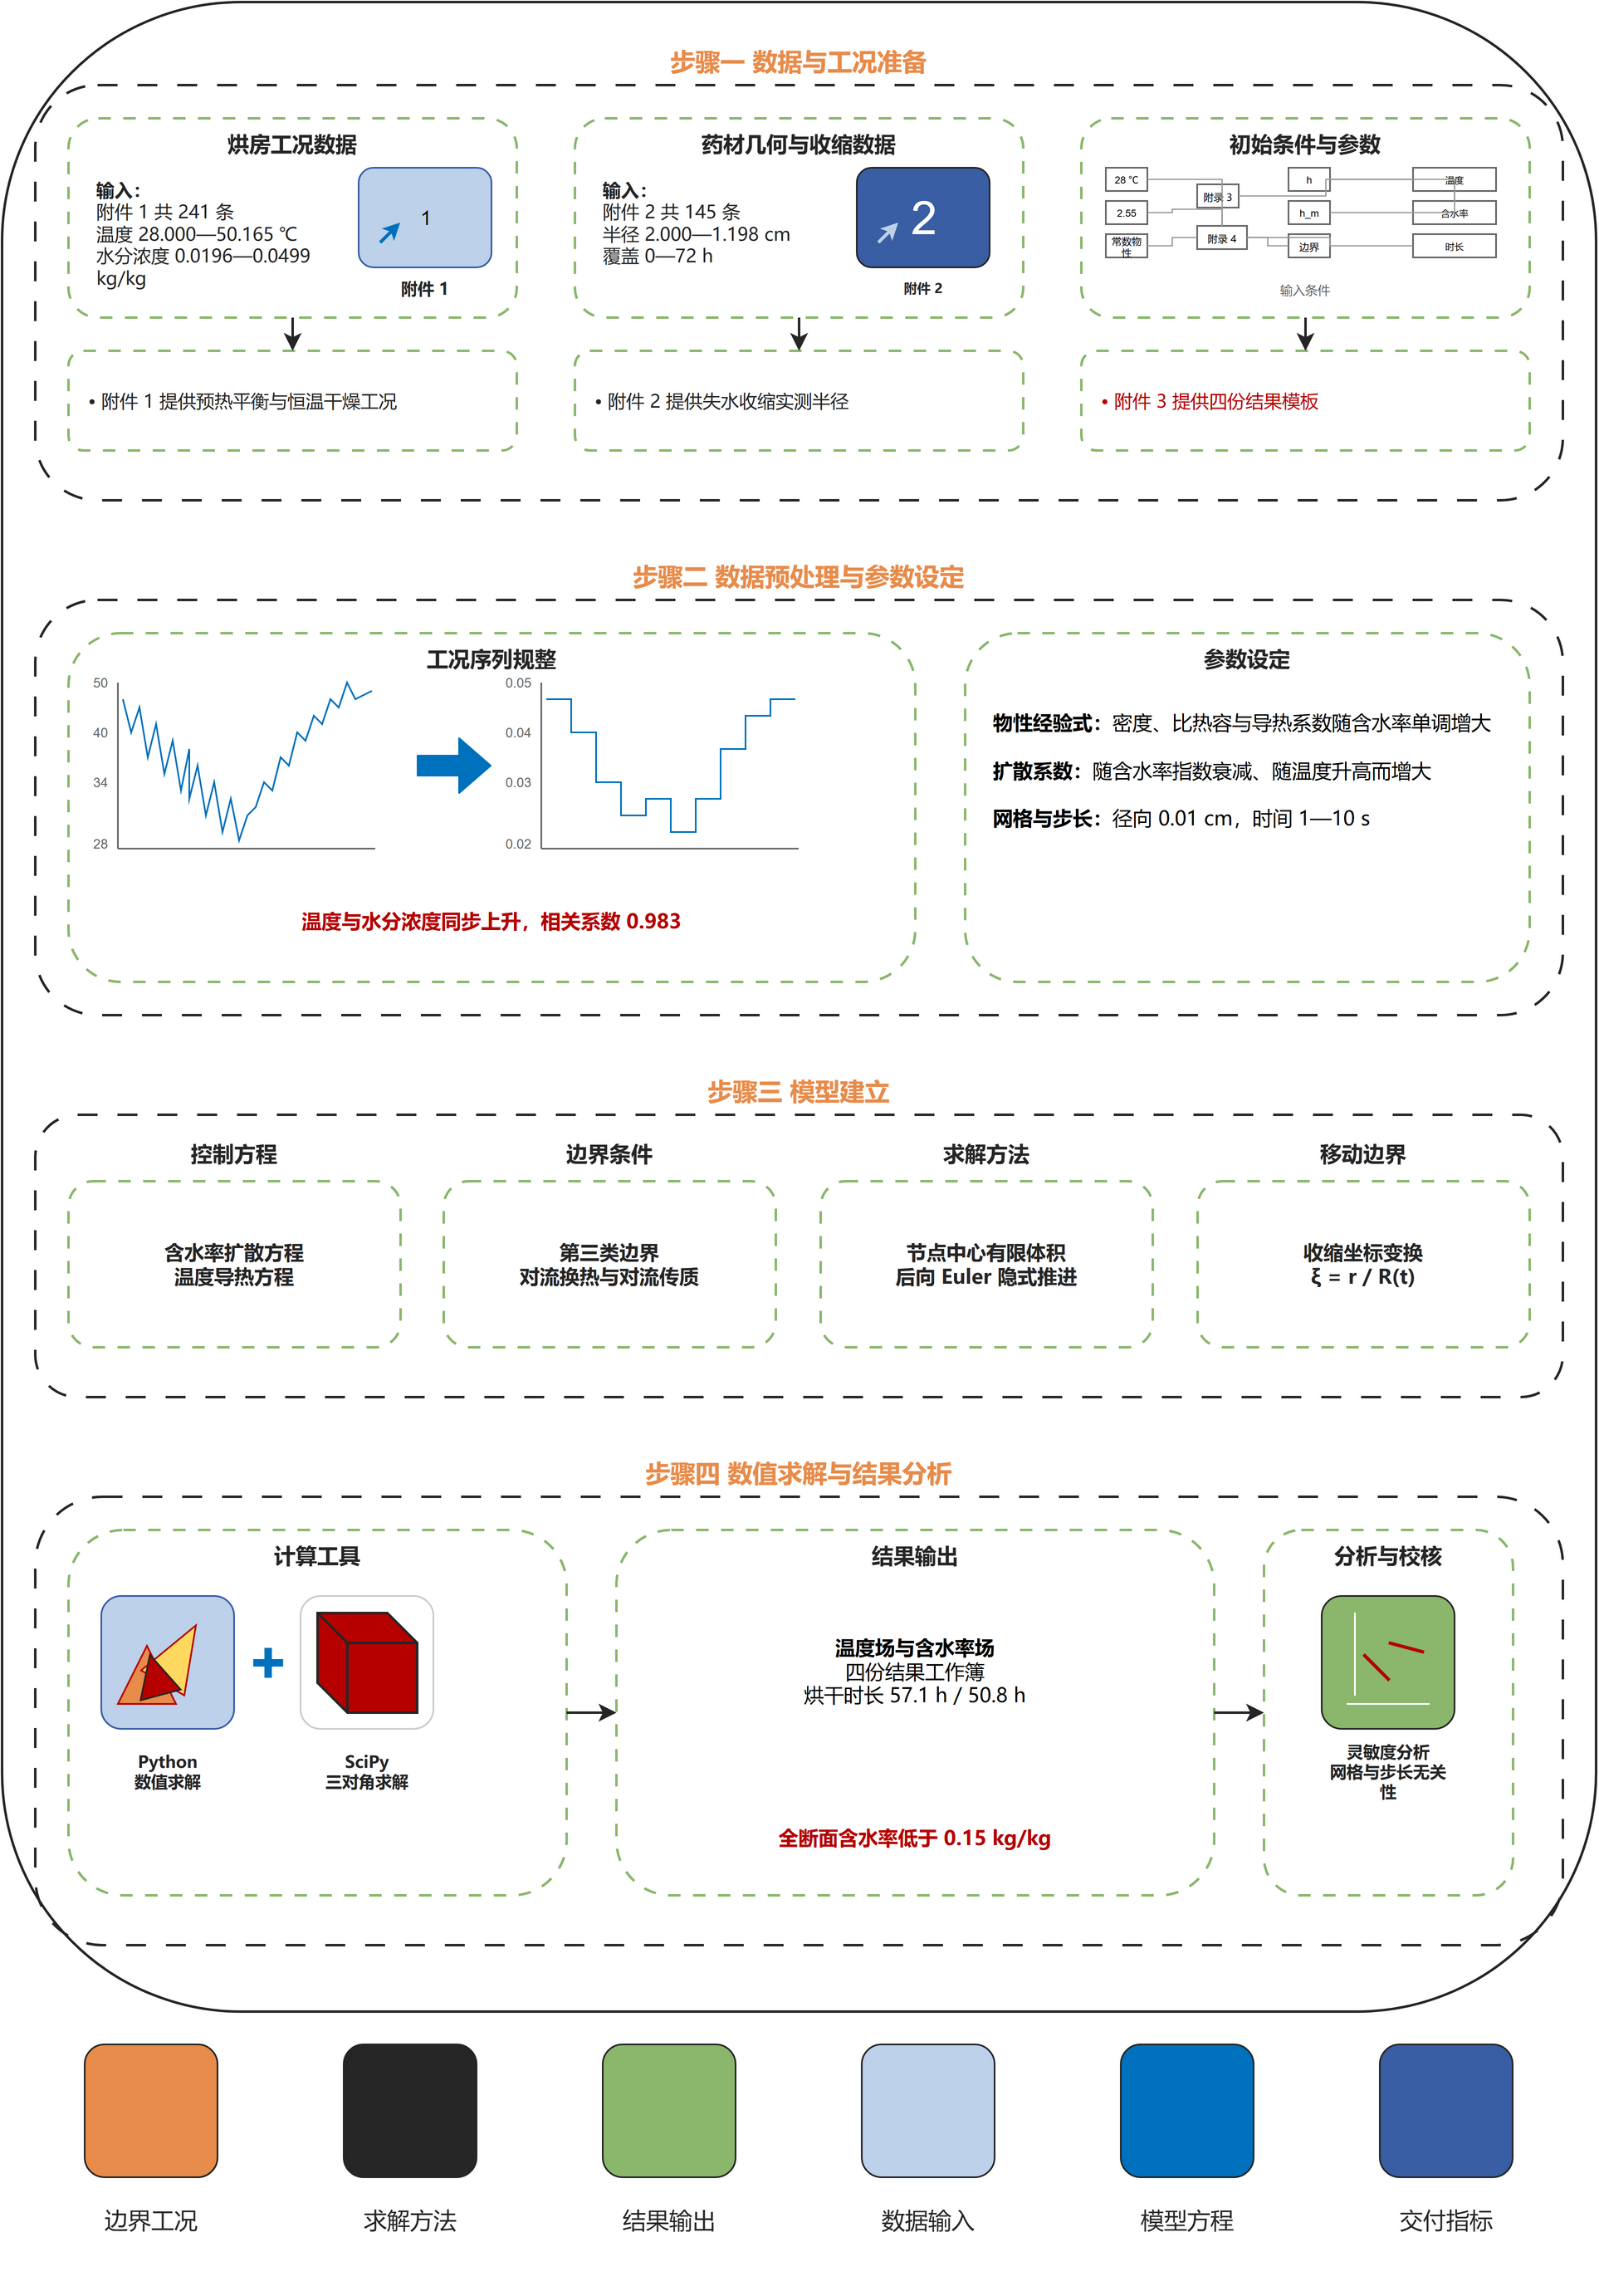
\includegraphics[width=0.86\textwidth]{../手绘图/技术路线图.png}
    \caption{论文技术路线图}
    \label{fig:roadmap}
\end{figure}

\section{模型假设}

\begin{enumerate}
    \item 药材视为均质、各向同性的圆柱形湿多孔介质，温度与含水率只沿半径方向变化，忽略轴向与周向梯度。
    \item 烘干开始前药材内部温度与含水率均匀，分别为 28 ℃ 与 2.55 kg/kg。
    \item 烘房空气充分混合，其温度与水分浓度在任意时刻沿空间均匀，附件 1 的相邻采样点之间按线性插值取连续工况。
    \item 预热平衡阶段药材尺寸不变，半径固定为 2 cm；恒温干燥阶段问题二与问题三仍沿用该假设，问题四按附件 2 的实测半径考虑收缩。
    \item 药材表面与烘房空气之间的换热与传质满足第三类边界条件，即表面通量正比于表面与空气之间的温差和浓度差。
    \item 问题一取常数物性；问题二与问题三取附录 3 的经验式；问题四取附录 4 的经验式。经验式中的温度以开尔文代入，输出统一换算为摄氏度。
    \item 附件 1 只覆盖 0 至 14400 s。14400 s 之后进入恒温干燥阶段，按题面所述两阶段参数不同，取附件 1 的末值 50.165 ℃ 与 0.049860 kg/kg 作为恒定边界工况。
    \item 问题四的收缩是各向同性的均匀收缩，任意时刻半径按同一比例缩小；半径由附件 2 的实测序列经保形插值重建，超过 72 h 后按最后实测值保持，不作外推。
    \item 干燥过程中不考虑药材开裂、成分迁移引起的物性突变以及水分在气相中的对流输运。
\end{enumerate}

\section{符号说明}

\begin{table}[H]
    \centering
    \caption{主要符号说明}
    \begin{tabular}{clc}
        \toprule
        符号 & 含义 & 单位 \\
        \midrule
        $r$ & 到药材中心的距离 & m \\
        $R$ & 药材半径 & m \\
        $t$ & 时间 & s \\
        $T$ & 药材温度 & ℃ \\
        $C$ & 干基含水率 & kg/kg \\
        $T_a$ & 烘房温度 & ℃ \\
        $C_a$ & 烘房水分浓度 & kg/kg \\
        $D$ & 水分浓度扩散系数 & m²/s \\
        $\rho$ & 药材密度 & kg/m³ \\
        $c_p$ & 药材比热容 & J/(kg·K) \\
        $k$ & 热传导系数 & W/(m·K) \\
        $h$ & 对流换热系数 & W/(m²·K) \\
        $h_m$ & 对流传质系数 & m/s \\
        $\xi$ & 无量纲径向坐标 & 1 \\
        $\dot R$ & 药材收缩速率 & m/s \\
        $C_{\mathrm{th}}$ & 烘干含水率判据 & kg/kg \\
        $t_{\mathrm{end}}$ & 烘干所需时间 & s \\
        \bottomrule
    \end{tabular}
\end{table}

\section{模型建立与求解}

\subsection{数据预处理}

附件 1 与附件 2 是全部建模依据。附件 1 的 241 条记录中，时间严格递增、无缺失、无重复，温度取值范围为 28.000 至 50.165 ℃，水分浓度取值范围为 0.019630 至 0.049860 kg/kg。两者的 Pearson 相关系数达到 0.983，说明升温与水分蒸发同步发生，烘房在预热平衡阶段同时经历升温与增湿，边界工况不能当作恒定值处理。附件 2 的 145 条记录中，半径由 2.000 cm 单调收缩到 1.198 cm，收缩幅度为 0.802 cm，且收缩速率在前期快速衰减、约 20 h 之后趋于零。

两份附件的量级差异决定了传质边界条件的写法。烘房水分浓度约为 10⁻² kg/kg，药材含水率约为 10⁰ kg/kg，两者不是同一尺度上的直接平衡量。若把表面含水率直接取为烘房水分浓度，会使表面瞬间变干，与预热平衡阶段的物理过程不符。因此本文采用浓度差驱动的对流边界条件，表面通量正比于表面含水率与烘房水分浓度之差，比例系数取题给的对流传质系数。

数据规整只做去重、缺失剔除与时间排序，不对原始数值作平滑、滤波或量纲换算。规整结果写入派生数据文件，供四个问题共用。附件 1 与附件 2 的关键特征如图~\ref{fig:eda} 所示，烘房温度与水分浓度同向上升且高度线性相关，药材半径的收缩速率在 20 h 后趋于零，这两点分别支撑了恒定边界工况假设与保形插值重建策略。

\begin{figure}[H]
    \centering
    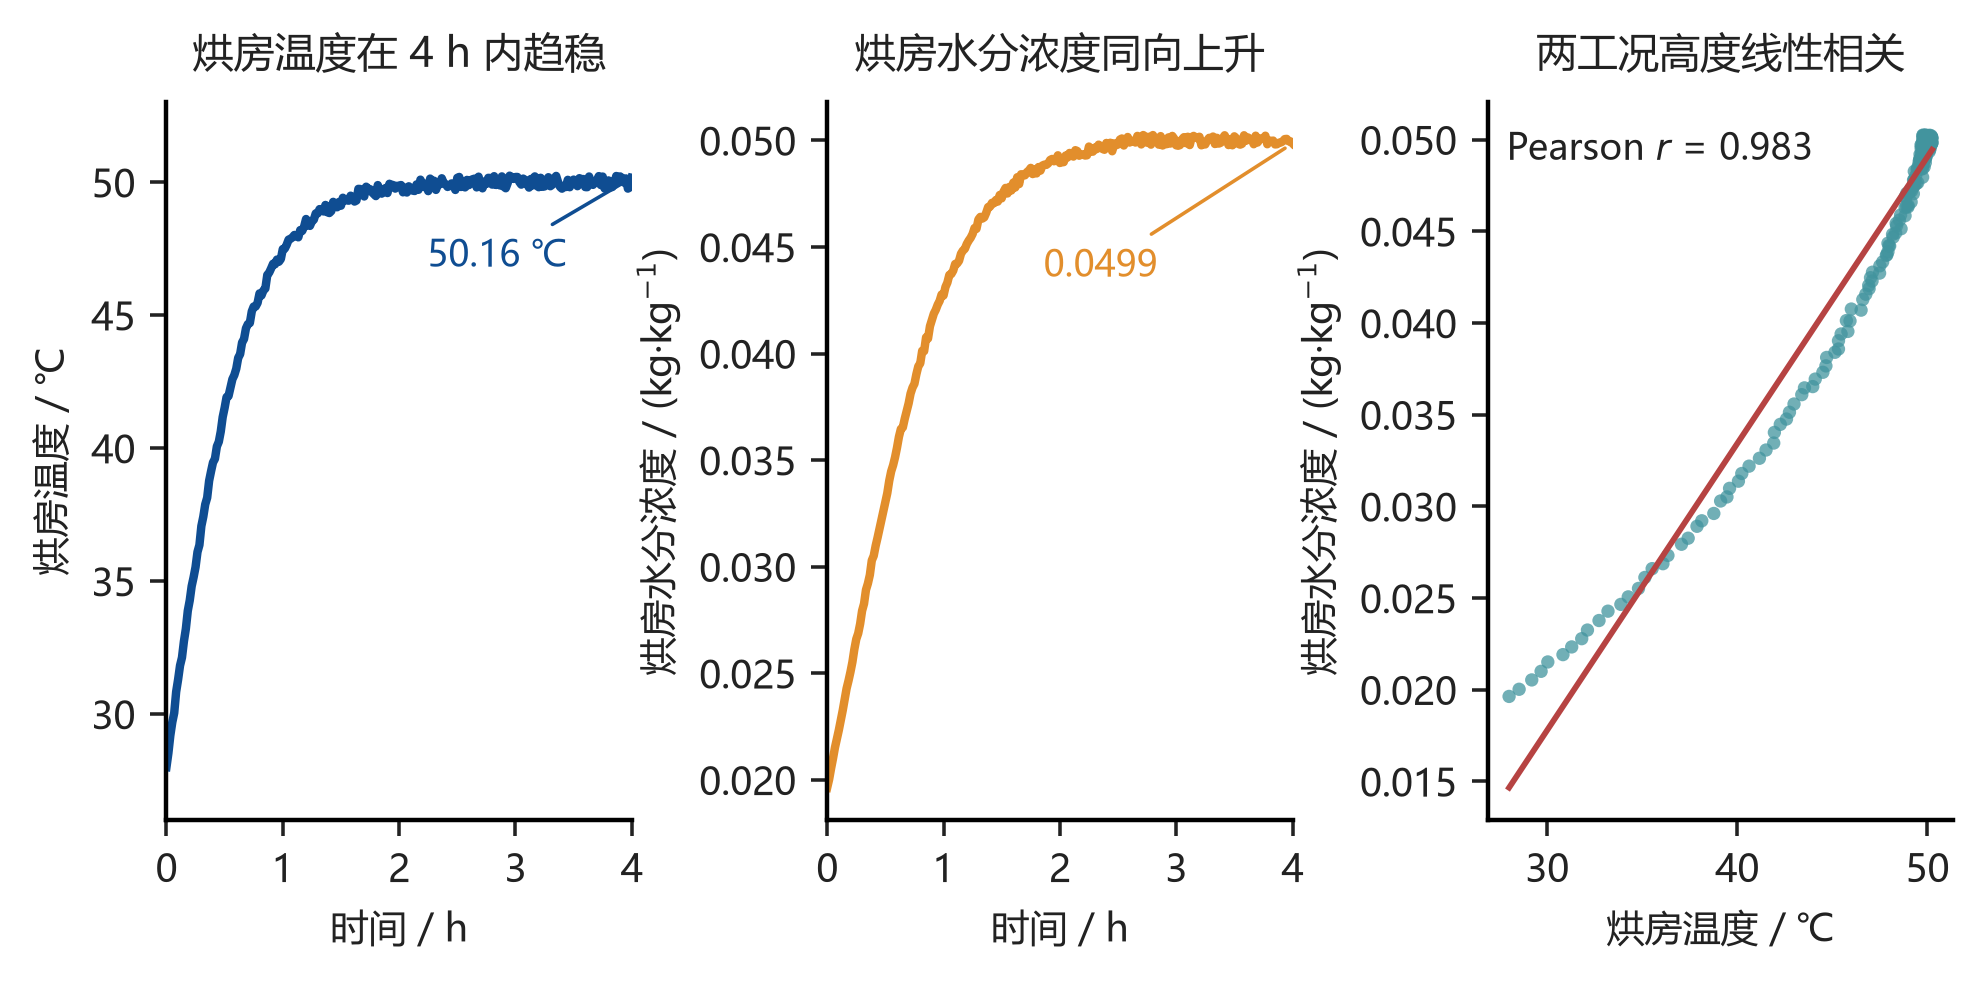
\includegraphics[width=0.86\textwidth]{../数据预处理/figures/fig_eda_ambient.png}
    \caption{烘房边界工况演化}
    \label{fig:eda}
\end{figure}

\subsection{问题一模型的建立与求解}

\subsubsection{控制方程与边界条件}

把药材视为半径 $R$ 的均质圆柱，取径向坐标 $r$，以干基含水率 $C(r,t)$ 与温度 $T(r,t)$ 为状态量。对半径 $r$ 处厚度为 $\mathrm{d}r$ 的薄圆环写水分守恒关系，单位时间进入圆环的水分由圆环内外两侧的通量差给出。圆柱的侧面积为 $2\pi r$，因此径向通量 $J$ 满足

\begin{equation}
\frac{\partial C}{\partial t} = \frac{1}{r}\frac{\partial}{\partial r}\left(D(C)\,r\frac{\partial C}{\partial r}\right)
\label{eq:q1mass}
\end{equation}

其中扩散系数按题给经验式取 $D(C)=7\times10^{-9}\exp(-0.89/C)$。式~\eqref{eq:q1mass} 的右端来自把通量 $J=-D\partial C/\partial r$ 代入守恒关系 $r\partial C/\partial t = -\partial(rJ)/\partial r$，除以 $r$ 后即得。由于 $D$ 随 $C$ 单调下降，含水率越低扩散越慢，方程是拟线性的。

同理写出能量守恒关系。薄圆环的热容为 $\rho c_p 2\pi r\,\mathrm{d}r$，导热通量为 $-k\partial T/\partial r$，得到

\begin{equation}
\rho c_p \frac{\partial T}{\partial t} = \frac{1}{r}\frac{\partial}{\partial r}\left(k\,r\frac{\partial T}{\partial r}\right)
\label{eq:q1heat}
\end{equation}

其中密度、比热容与热传导系数取附录 2 的常数值。式~\eqref{eq:q1mass} 与式~\eqref{eq:q1heat} 形式相同，说明在常数物性下温度场与含水率场的演化机制一致，差别只在扩散系数的量级。

边界条件在药材表面与对称轴上分别给出。表面与烘房空气之间同时发生对流换热与对流传质，通量正比于表面与空气的差值；对称轴处通量为零。于是

\begin{equation}
-D\frac{\partial C}{\partial r}\bigg|_{r=R}=h_m\left(C\big|_{r=R}-C_a(t)\right),\qquad
-k\frac{\partial T}{\partial r}\bigg|_{r=R}=h\left(T\big|_{r=R}-T_a(t)\right)
\label{eq:q1bc}
\end{equation}

\begin{equation}
\frac{\partial C}{\partial r}\bigg|_{r=0}=0,\qquad
\frac{\partial T}{\partial r}\bigg|_{r=0}=0
\label{eq:q1sym}
\end{equation}

其中 $T_a(t)$ 与 $C_a(t)$ 由附件 1 线性插值得到。式~\eqref{eq:q1bc} 中的传质通量用含水率差驱动，而不是用绝对湿度差驱动，这与附件 1 与药材含水率的量级差异相匹配。

\subsubsection{特征时间与机理判断}

在判断含水率场能否在 1800 s 内发生整体变化之前，需要比较热扩散与质量扩散的特征时间。定义

\begin{equation}
\tau_T=\frac{R^2}{k/(\rho c_p)},\qquad
\tau_C=\frac{R^2}{D_0}
\label{eq:q1tau}
\end{equation}

取 $R=0.02$ m，热扩散率 $k/(\rho c_p)=1.69\times10^{-7}$ m²/s，得 $\tau_T=2.4\times10^{3}$ s 的量级；取干燥初期的 $D_0=4.9\times10^{-9}$ m²/s，得 $\tau_C=8.2\times10^{4}$ s。两者相差约 34 倍，说明在 1800 s 内热量足以穿透整个半径，而水分只能在外层形成薄薄的扰动层。

表面传质阻力与内部扩散阻力的比值由质量 Biot 数刻画，即 $\mathrm{Bi}_m=h_mR/D_0=3.2$。该值介于 1 与 10 之间，说明外部传质阻力与内部扩散阻力处于同一量级，表面含水率既不会瞬间等于烘房水分浓度，也不会被内部完全钳制，而是稳定在两者之间。这一判断在数值结果中得到验证。

\subsubsection{有限体积离散与求解流程}

在 $[0,R]$ 上取 $N+1$ 个节点，节点间距 $\Delta r=R/N$，节点半径 $r_j=j\Delta r$。对节点 $j$ 周围的控制体 $[r_j-\Delta r/2,\,r_j+\Delta r/2]$ 积分式~\eqref{eq:q1mass}，用界面上的扩散系数平均值近似界面通量，得到半离散方程

\begin{equation}
\frac{\mathrm{d}C_j}{\mathrm{d}t}=\frac{r_{j+1/2}D_{j+1/2}\dfrac{C_{j+1}-C_j}{\Delta r}-r_{j-1/2}D_{j-1/2}\dfrac{C_j-C_{j-1}}{\Delta r}}{r_j\Delta r}
\label{eq:q1fv}
\end{equation}

其中 $r_{j\pm1/2}=r_j\pm\Delta r/2$，$D_{j\pm1/2}$ 取相邻节点扩散系数的算术平均。在对称轴 $j=0$ 处利用洛必达法则把式~\eqref{eq:q1mass} 的右端化为 $4D_{1/2}(C_1-C_0)/\Delta r^2$，在表面 $j=N$ 处用式~\eqref{eq:q1bc} 替换外侧通量。温度方程按同样的方式离散，只需把 $D$ 换成 $k/(\rho c_p)$、把 $h_m$ 换成 $h/(\rho c_p)$。

时间推进采用后向 Euler 格式，并把上一时刻的扩散系数冻结在界面系数中，使每一步成为三对角线性系统。求解流程如下。

\begin{algorithm}[H]
\caption{问题一的热湿耦合求解流程}
\begin{algorithmic}[1]
\Require 网格参数 $N$、时间步长 $\Delta t$、初始条件 $T_0$ 与 $C_0$、物性常数
\Ensure 每个时刻的温度场与含水率场
\State \stepfont{1} 由附件 1 构造插值函数 $T_a(t)$ 与 $C_a(t)$
\State \stepfont{2} 初始化 $T_j$ 与 $C_j$，生成节点半径与界面半径
\State \stepfont{3} 由当前 $C_j$ 计算界面扩散系数 $D_{j\pm1/2}$
\State \stepfont{4} 组装含水率方程的三对角系数并求解，得到新的 $C_j$
\State \stepfont{5} 组装温度方程的三对角系数并求解，得到新的 $T_j$
\State \stepfont{6} 判断是否达到终止时间，未达到则返回第 3 步
\State \stepfont{7} \Return 各时刻的温度场与含水率场
\end{algorithmic}
\end{algorithm}

本文取 $N=200$，即径向步长 0.01 cm，使 0 至 2.0 cm 范围内每隔 0.1 cm 的输出点恰好落在节点上，避免插值带来的额外误差。时间步长取 1 s，与结果工作簿要求的输出间隔一致。

\subsubsection{结果与分析}

计算得到 1800 s 时刻表面温度为 36.7863 ℃、中心温度为 33.5765 ℃，表面含水率为 1.5104 kg/kg、中心含水率为 2.5500 kg/kg。温度场的演化如图~\ref{fig:q1temp} 所示，等值线由表面向中心逐层推进，30 min 时表面与中心温差为 3.2098 ℃。含水率场的演化如图~\ref{fig:q1moist} 所示，扰动集中在靠近表面的薄层内，等值线密集排列，说明该层内的梯度远大于内部。

\begin{figure}[H]
    \centering
    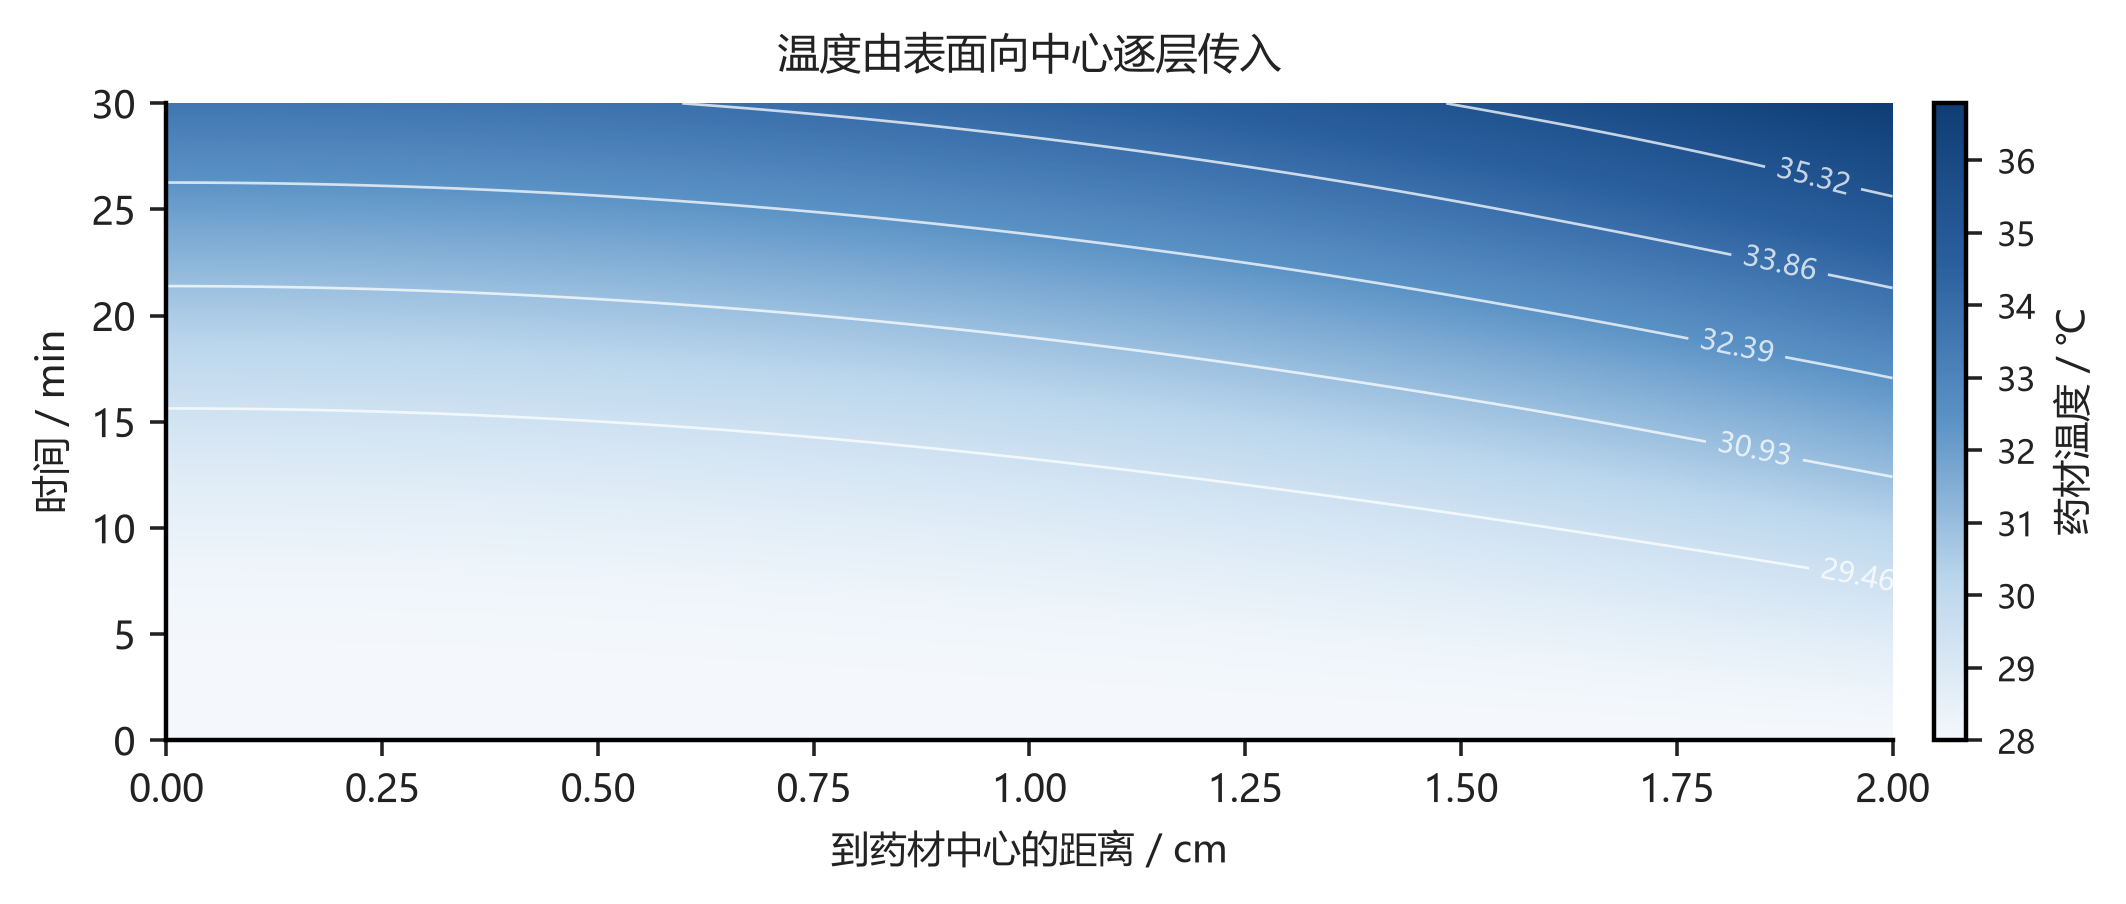
\includegraphics[width=0.86\textwidth]{../Q1/figures/fig_q1_temperature_field.png}
    \caption{预热平衡阶段温度场演化}
    \label{fig:q1temp}
\end{figure}

\begin{figure}[H]
    \centering
    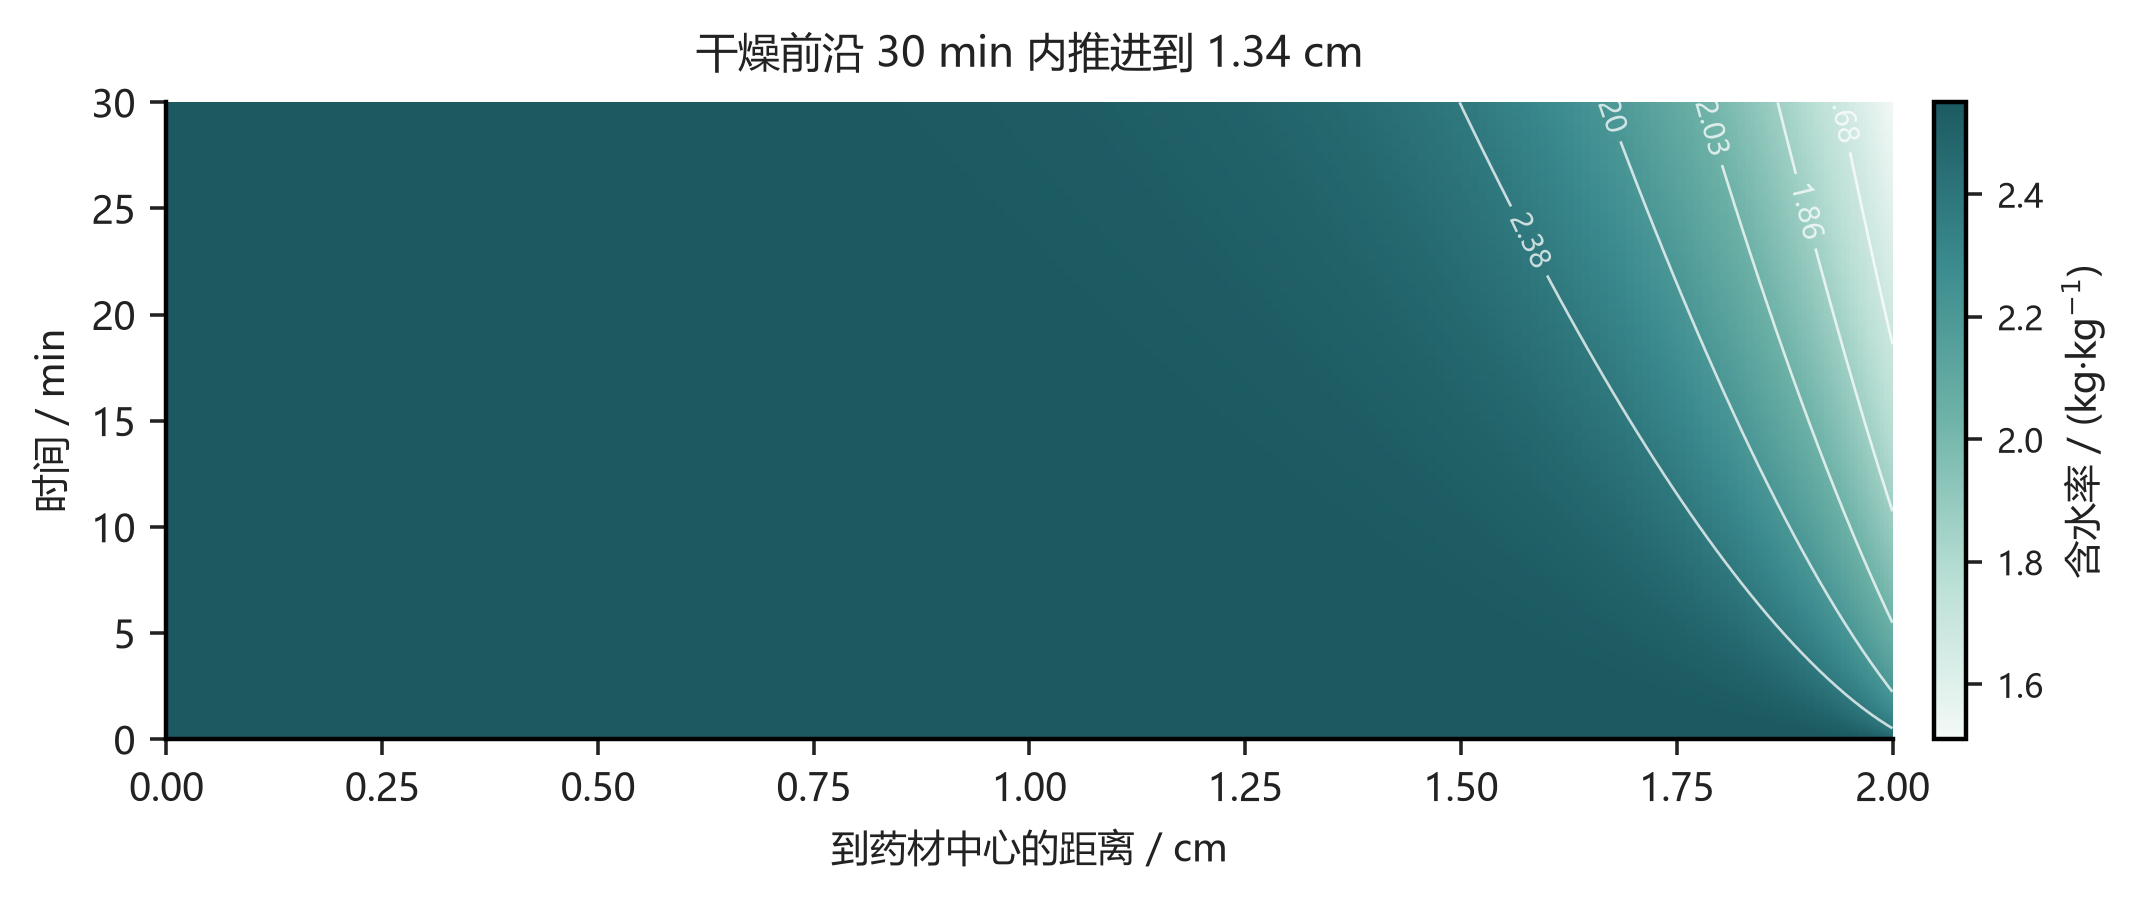
\includegraphics[width=0.86\textwidth]{../Q1/figures/fig_q1_moisture_field.png}
    \caption{预热平衡阶段含水率场演化}
    \label{fig:q1moist}
\end{figure}

特征时刻的含水率剖面与特征点温度曲线如图~\ref{fig:q1prof} 所示。剖面在 $r=1.0$ cm 以内几乎重合，在 $r=1.5$ cm 以外明显张开，与特征时间分析给出的扰动深度一致。温度曲线则显示表面与中心同步上升，中心温度在 6 min 之后开始加速，说明热量已经穿透整个半径。

\begin{figure}[H]
    \centering
    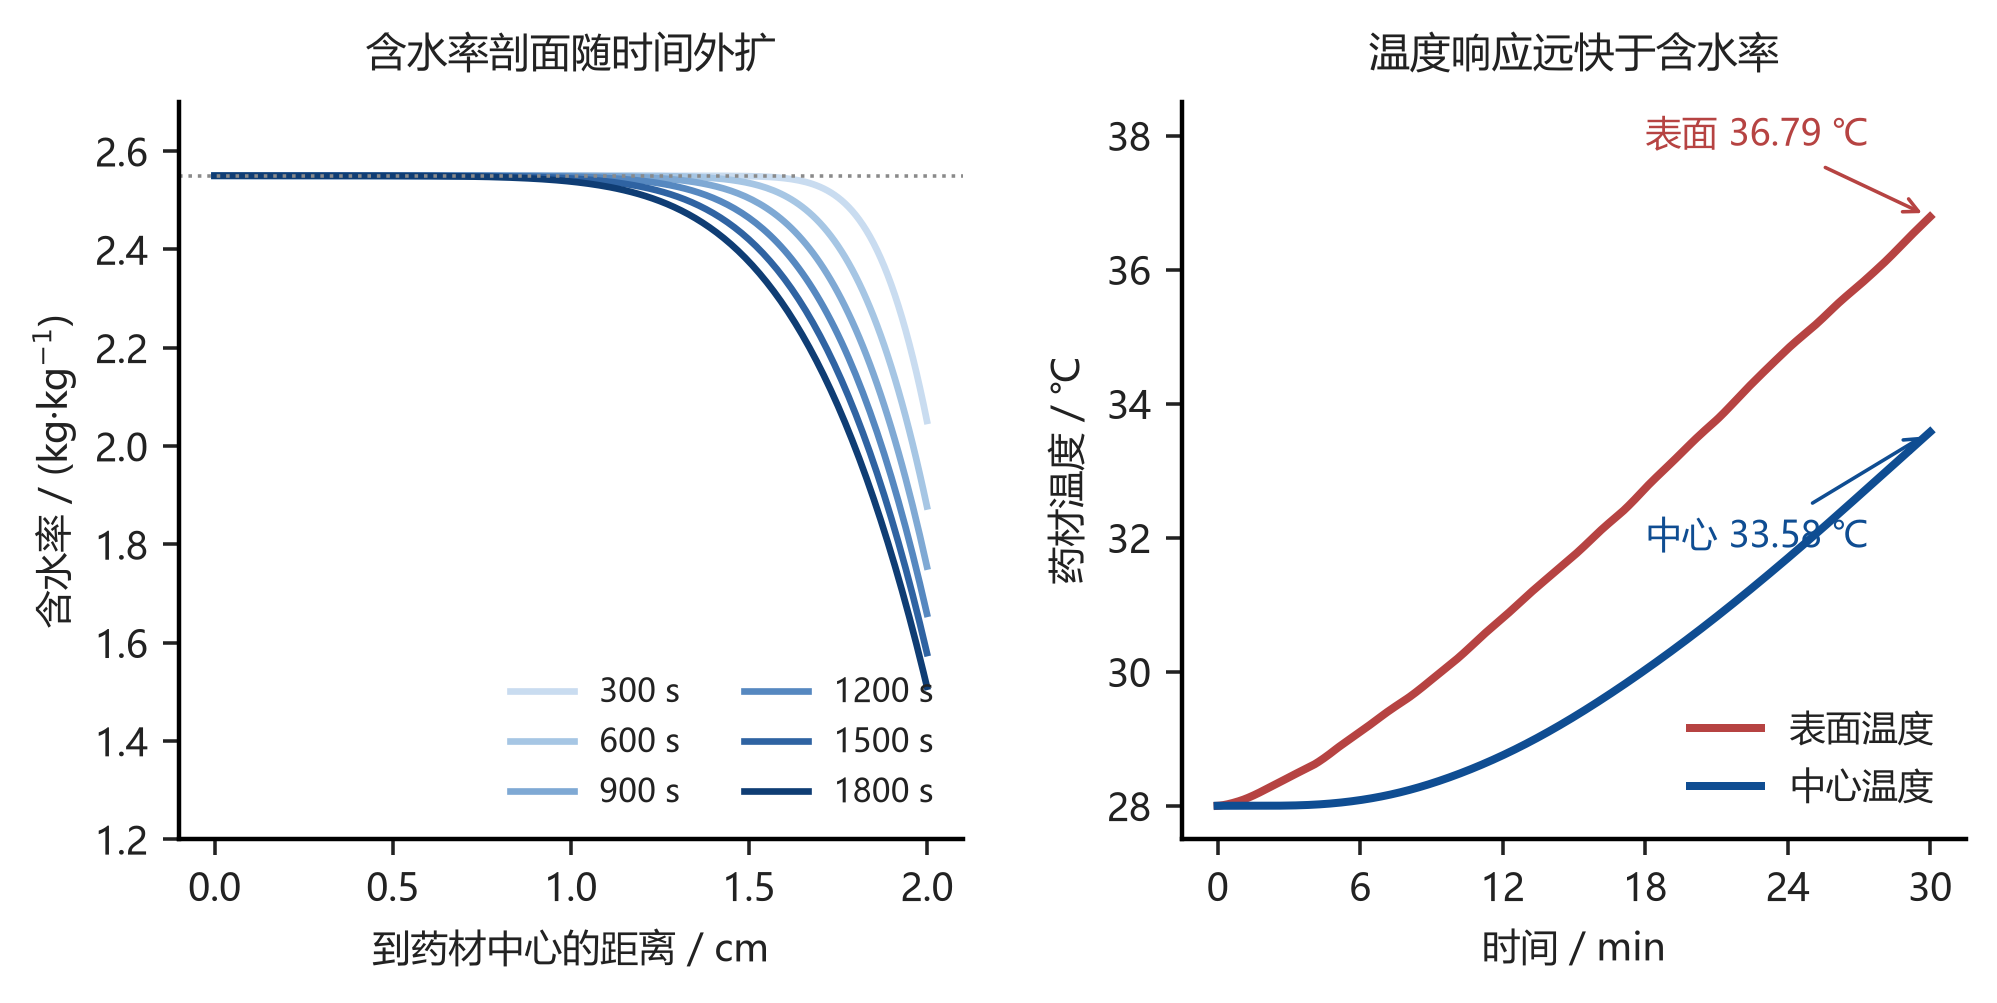
\includegraphics[width=0.86\textwidth]{../Q1/figures/fig_q1_profiles.png}
    \caption{特征剖面与特征点温度}
    \label{fig:q1prof}
\end{figure}

温度对时间与半径的耦合依赖如图~\ref{fig:q1surf} 所示。曲面在时间方向上先陡后缓，在半径方向上由表面向中心单调下降，整体呈现“表面先行、中心滞后”的形态。该形态与式~\eqref{eq:q1tau} 给出的时间尺度比一致。

\begin{figure}[H]
    \centering
    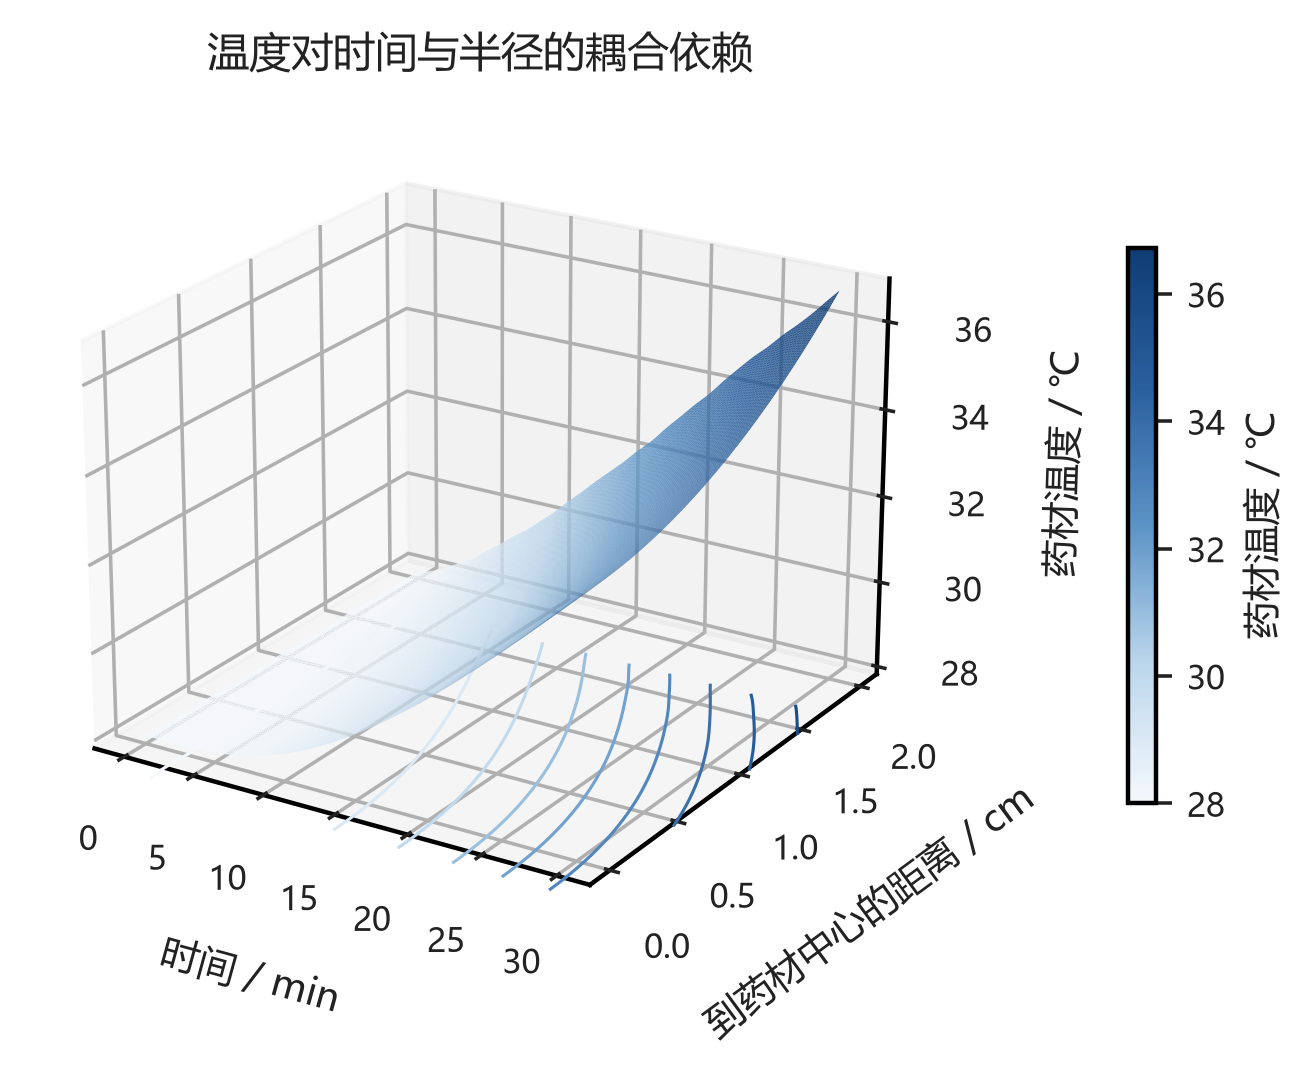
\includegraphics[width=0.86\textwidth]{../Q1/figures/fig_q1_surface3d.png}
    \caption{温度对时间与半径的响应面}
    \label{fig:q1surf}
\end{figure}

按题目要求的格式整理结果，温度见表~\ref{tab:q1t}，水分浓度见表~\ref{tab:q1c}。

\begin{table}[H]
    \centering
    \caption{30 分钟内药材的温度}
    \begin{tabular}{cccccc}
        \toprule
        \makecell{时间/s} & \multicolumn{5}{c}{到药材中心的距离/cm} \\
        \cmidrule(lr){2-6}
         & 0 & 0.5 & 1 & 1.5 & 2 \\
        \midrule
        100 & 28.0001 & 28.0004 & 28.0043 & 28.0332 & 28.1807 \\
        300 & 28.0415 & 28.0643 & 28.1523 & 28.3691 & 28.8498 \\
        600 & 28.4549 & 28.5376 & 28.8054 & 29.3171 & 30.1661 \\
        900 & 29.3262 & 29.4601 & 29.8771 & 30.6174 & 31.7313 \\
        1200 & 30.5445 & 30.7115 & 31.2239 & 32.1139 & 33.4286 \\
        1500 & 31.9974 & 32.1883 & 32.7674 & 33.7473 & 35.1209 \\
        1800 & 33.5765 & 33.7732 & 34.3653 & 35.3631 & 36.7863 \\
        \bottomrule
    \end{tabular}
    \label{tab:q1t}
\end{table}

\begin{table}[H]
    \centering
    \caption{30 分钟内药材的水分浓度}
    \begin{tabular}{cccccc}
        \toprule
        \makecell{时间/s} & \multicolumn{5}{c}{到药材中心的距离/cm} \\
        \cmidrule(lr){2-6}
         & 0 & 0.5 & 1 & 1.5 & 2 \\
        \midrule
        100 & 2.5500 & 2.5500 & 2.5500 & 2.5500 & 2.2478 \\
        300 & 2.5500 & 2.5500 & 2.5500 & 2.5492 & 2.0512 \\
        600 & 2.5500 & 2.5500 & 2.5500 & 2.5352 & 1.8772 \\
        900 & 2.5500 & 2.5500 & 2.5497 & 2.5045 & 1.7549 \\
        1200 & 2.5500 & 2.5500 & 2.5482 & 2.4645 & 1.6587 \\
        1500 & 2.5500 & 2.5499 & 2.5445 & 2.4206 & 1.5789 \\
        1800 & 2.5500 & 2.5497 & 2.5383 & 2.3755 & 1.5104 \\
        \bottomrule
    \end{tabular}
    \label{tab:q1c}
\end{table}

表中的数值给出三点结论。表层含水率的下降幅度为 1.0396 kg/kg，占初始含水率的四成，说明预热平衡阶段并非“只升温不失水”。$r=0$ 与 $r=0.5$ cm 两列在 1800 s 内基本不变，中心含水率始终为 2.5500 kg/kg，说明干燥扰动尚未到达中心。按含水率变化超过 0.001 kg/kg 判定，扰动深度为 1.34 cm，占半径的 67\%，与 $\sqrt{\tau_C}$ 与 $\sqrt{\tau_T}$ 的比值给出的估计相符。

\subsection{问题二模型的建立与求解}

\subsubsection{物性经验式与耦合机理}

问题二把常数物性替换为附录 3 的经验式，密度、比热容与热传导系数均随含水率单调增大，扩散系数同时随含水率与温度变化。控制方程形式不变，但系数不再是常数，能量方程改写为

\begin{equation}
\rho(C)\,c_p(C)\frac{\partial T}{\partial t}=\frac{1}{r}\frac{\partial}{\partial r}\left(k(C)\,r\frac{\partial T}{\partial r}\right)
\label{eq:q2heat}
\end{equation}

含水率方程仍为式~\eqref{eq:q1mass}，但扩散系数改为 $D(C,T)=2.4\times10^{-3}\exp(-0.45/C)\exp(-3850/T)$。该式包含两个因子，前一个因子随含水率下降而指数衰减，后一个因子随温度升高而增大。两者的乘积决定了干燥速率随时间的走向：升温提高扩散能力，失水降低扩散能力，前期升温占优，后期失水占优，因此干燥速率必然出现由升转降的拐点。

各物性随含水率的变化如图~\ref{fig:q2prop} 所示。密度由 650 增至 976 kg/m³，比热容由 1580 增至 3390 J/(kg·K)，热传导系数由 0.22 增至 0.46 W/(m·K)，三者都随含水率单调上升。扩散系数在 50 ℃ 下由 2.5×10⁻⁹ 降到 4.9×10⁻¹⁰ m²/s，跨越约 5 倍，且在含水率低于 0.3 kg/kg 之后下降得更为陡峭。这一非均匀衰减正是后期干燥变慢的直接原因。

\begin{figure}[H]
    \centering
    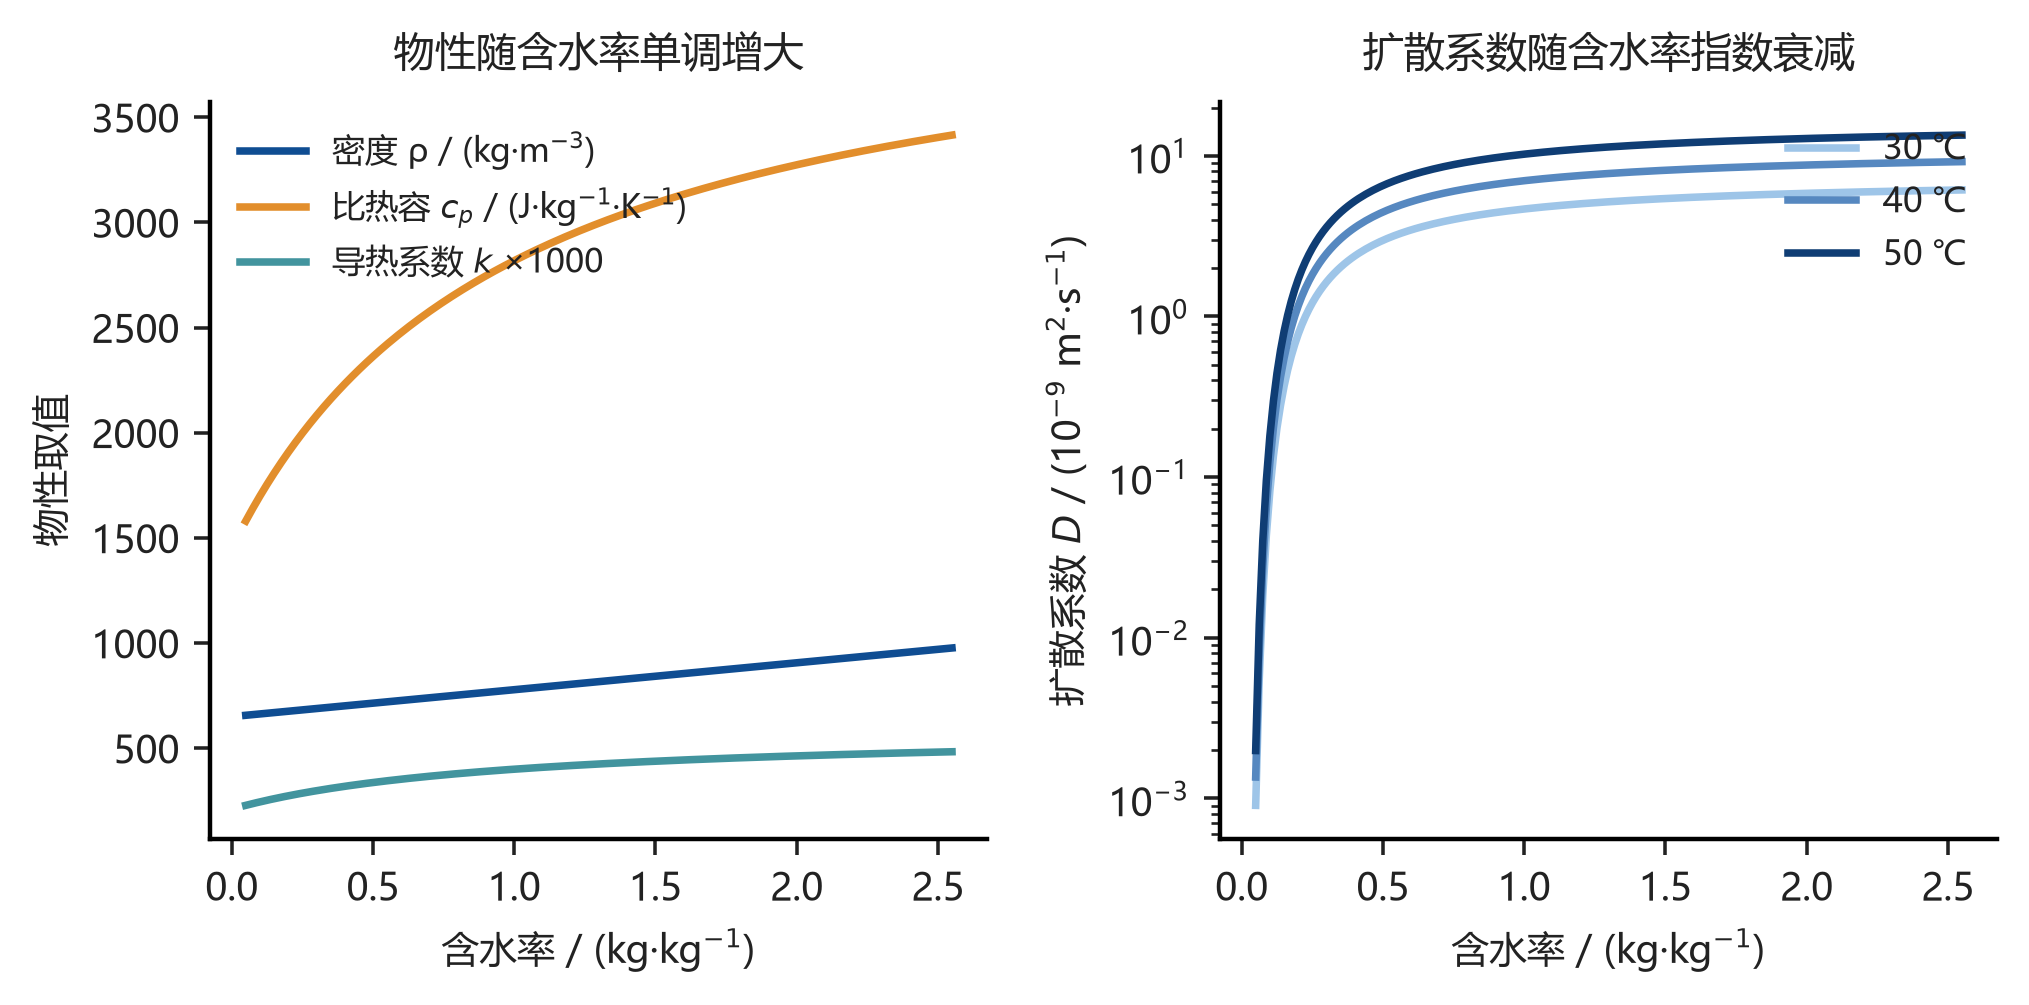
\includegraphics[width=0.86\textwidth]{../Q2/figures/fig_q2_properties.png}
    \caption{物性与扩散系数随含水率变化}
    \label{fig:q2prop}
\end{figure}

\subsubsection{两阶段边界工况的衔接}

附件 1 只覆盖 0 至 14400 s，而整个烘干过程持续 2 至 3 天。题面说明预热平衡与恒温干燥两个阶段的参数有所不同，但没有给出第二阶段的实测工况。本文按题面表述把 14400 s 之后的烘房工况固定为附件 1 的末值，即 $T_a=50.165$ ℃、$C_a=0.049860$ kg/kg。该处理保证了边界工况在 14400 s 处连续，不会引入人为跳变，同时在 3 h 内完全落在附件 1 的覆盖范围内，不影响问题二的结果。对于问题三与问题四，该处理相当于假设恒温干燥阶段的烘房能够稳定维持末值工况，属于建模假设，已在假设 7 中标注。

边界工况的连续性对数值求解有直接影响。若在 14400 s 处直接切换为不同的温度或湿度，表面的通量会发生跳变，进而在含水率剖面上留下折点。本文采用末值保持的方式，使 $T_a$ 与 $C_a$ 的一阶导在切换点两侧均为零，剖面保持光滑。

\subsubsection{数值实现与稳定性}

离散格式与问题一相同，差别在于每一步都要用当前含水率与温度重新计算物性系数。把系数取上一时刻的值相当于对非线性方程做一次 Picard 线性化，误差为 $O(\Delta t)$，与后向 Euler 格式本身的精度同阶，不会降低整体精度。由于后向 Euler 格式无条件稳定，时间步长只受精度约束。本文取时间步长 1 s，与结果工作簿要求的输出间隔一致，共推进 10800 步。

热扩散率在含水率下降的过程中由 $1.69\times10^{-7}$ 降到 $1.06\times10^{-7}$ m²/s，变化不超过两倍，因此温度场的演化始终处于快变过程；质量扩散系数由 $5.6\times10^{-9}$ 降到 $2.2\times10^{-9}$ m²/s，变化也不超过三倍。两者的比值维持在 30 以上，说明“温度先均匀、含水率后均匀”的层次结构在 3 h 内保持成立。

\subsubsection{结果与分析}

计算得到 3 h 时刻表面温度为 50.0048 ℃、中心温度为 49.9065 ℃，表面含水率为 1.0070 kg/kg、中心含水率为 1.7601 kg/kg。温度场的演化如图~\ref{fig:q2temp} 所示，等值线在 2 h 之后几乎垂直于半径方向，说明温度已经接近均匀，与烘房温度的差值仅为 0.2585 ℃。含水率场的演化如图~\ref{fig:q2moist} 所示，干燥前沿在 3 h 内推进到距中心约 1.1 cm，比问题一的 30 min 推进深度大得多，但中心区域仍有 1.7601 kg/kg 的含水率。

\begin{figure}[H]
    \centering
    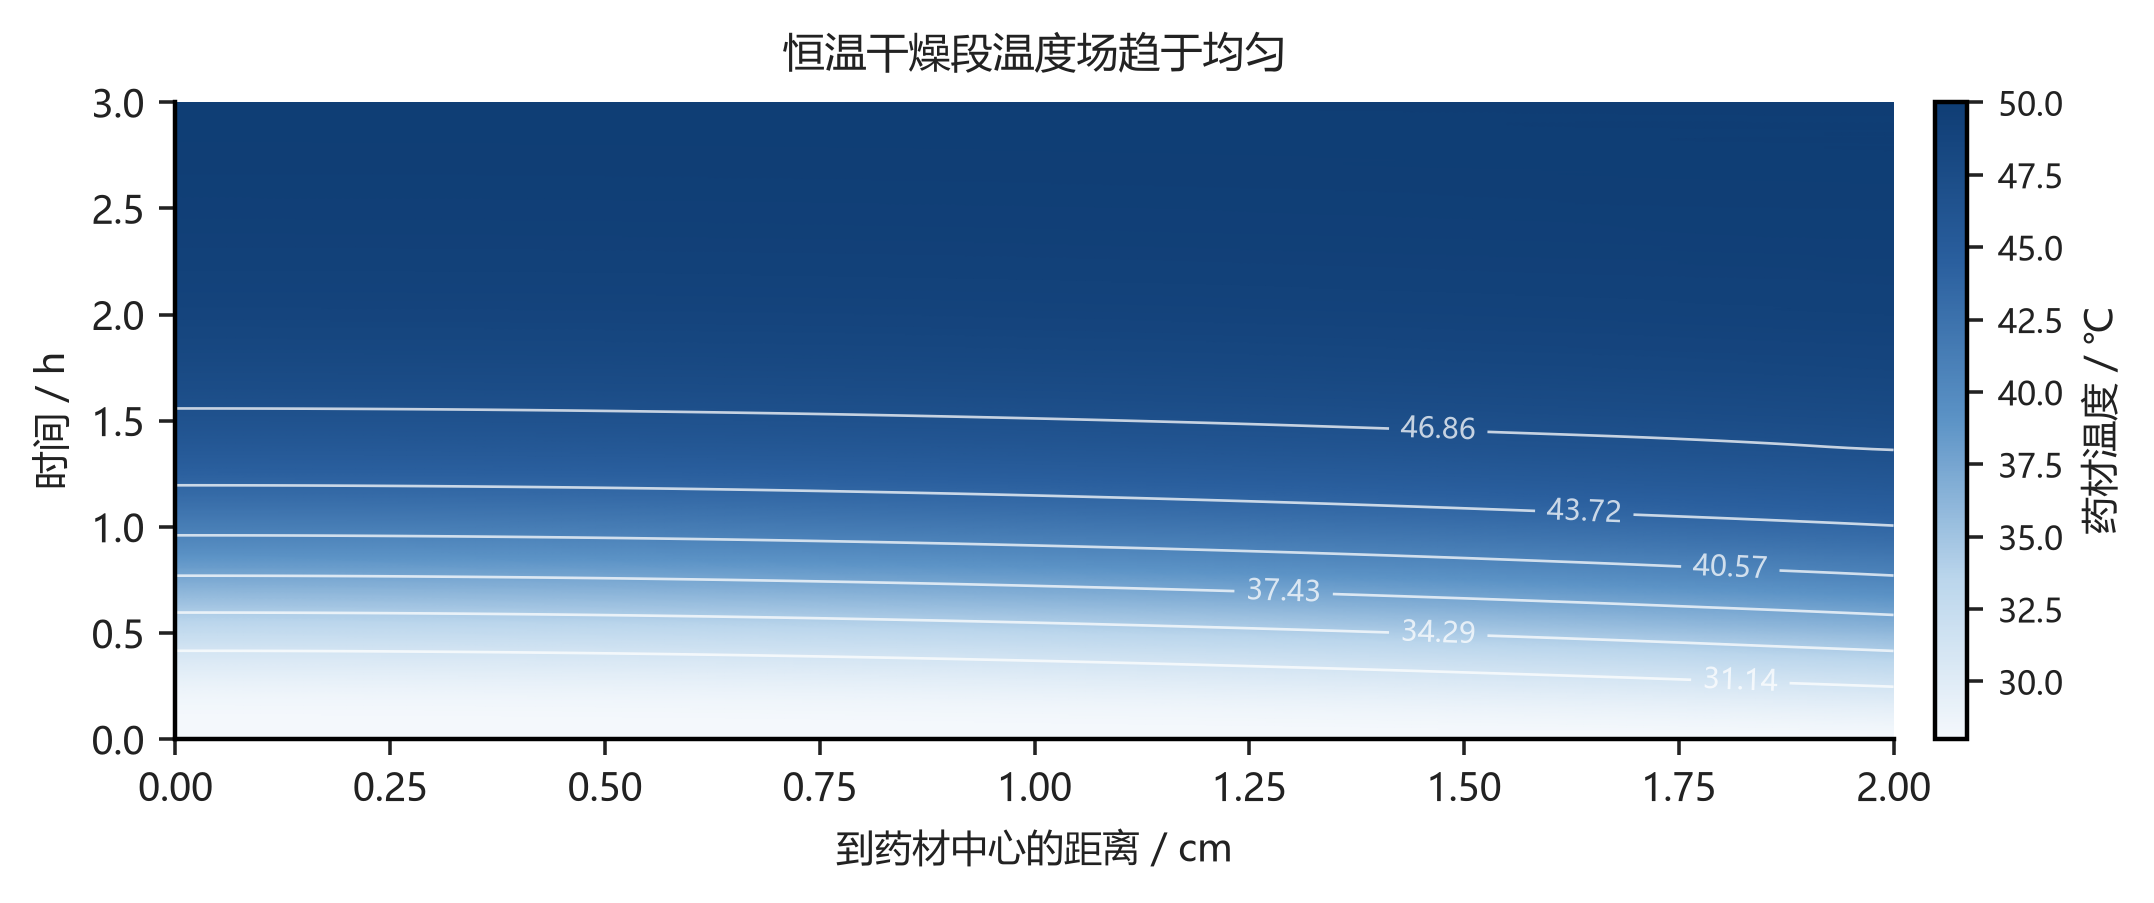
\includegraphics[width=0.86\textwidth]{../Q2/figures/fig_q2_temperature_field.png}
    \caption{恒温干燥阶段温度场演化}
    \label{fig:q2temp}
\end{figure}

\begin{figure}[H]
    \centering
    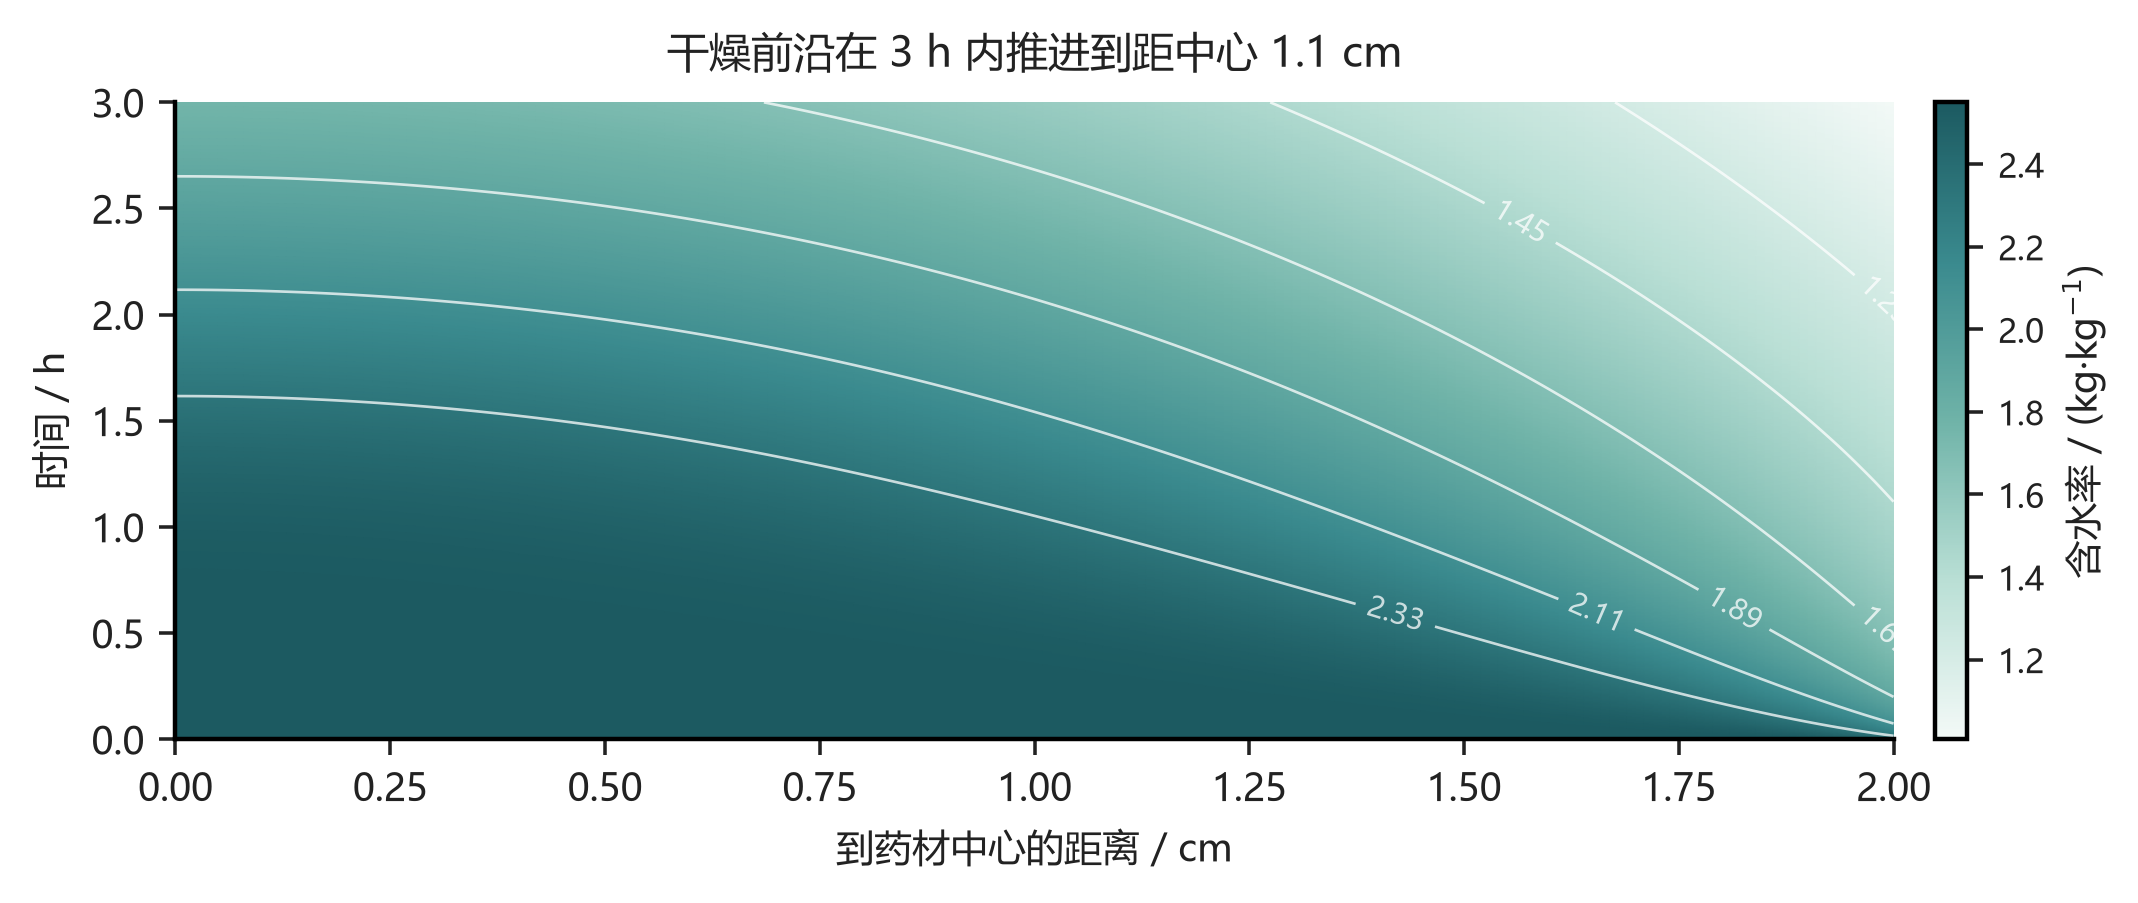
\includegraphics[width=0.86\textwidth]{../Q2/figures/fig_q2_moisture_field.png}
    \caption{恒温干燥阶段含水率场演化}
    \label{fig:q2moist}
\end{figure}

按题目要求的格式整理结果，温度见表~\ref{tab:q2t}，水分浓度见表~\ref{tab:q2c}。

\begin{table}[H]
    \centering
    \caption{3 小时内药材的温度}
    \begin{tabular}{cccccc}
        \toprule
        \makecell{时间/h} & \multicolumn{5}{c}{到药材中心的距离/cm} \\
        \cmidrule(lr){2-6}
         & 0 & 0.5 & 1 & 1.5 & 2 \\
        \midrule
        0.5 & 32.5459 & 32.7546 & 33.3851 & 34.4422 & 35.8769 \\
        1.0 & 41.1639 & 41.3376 & 41.8435 & 42.6319 & 43.6372 \\
        1.5 & 46.4761 & 46.5569 & 46.7900 & 47.1490 & 47.5847 \\
        2.0 & 48.7919 & 48.8240 & 48.9162 & 49.0573 & 49.2321 \\
        2.5 & 49.6151 & 49.6242 & 49.6490 & 49.6841 & 49.7559 \\
        3.0 & 49.9065 & 49.9113 & 49.9274 & 49.9576 & 50.0048 \\
        \bottomrule
    \end{tabular}
    \label{tab:q2t}
\end{table}

\begin{table}[H]
    \centering
    \caption{3 小时内药材的水分浓度}
    \begin{tabular}{cccccc}
        \toprule
        \makecell{时间/h} & \multicolumn{5}{c}{到药材中心的距离/cm} \\
        \cmidrule(lr){2-6}
         & 0 & 0.5 & 1 & 1.5 & 2 \\
        \midrule
        0.5 & 2.5499 & 2.5488 & 2.5249 & 2.3239 & 1.6536 \\
        1.0 & 2.5237 & 2.4917 & 2.3528 & 2.0204 & 1.4790 \\
        1.5 & 2.3777 & 2.3173 & 2.1277 & 1.8005 & 1.3534 \\
        2.0 & 2.1608 & 2.0994 & 1.9175 & 1.6243 & 1.2337 \\
        2.5 & 1.9485 & 1.8933 & 1.7310 & 1.4699 & 1.1168 \\
        3.0 & 1.7601 & 1.7110 & 1.5661 & 1.3309 & 1.0070 \\
        \bottomrule
    \end{tabular}
    \label{tab:q2c}
\end{table}

表~\ref{tab:q2t} 显示中心温度在前 30 min 内只升到 32.5459 ℃，而在 1 h 时已跳到 41.1639 ℃，说明升温过程存在明显的加速段，原因是表面温度升高后温差驱动的热流增大。表~\ref{tab:q2c} 显示 3 h 内表面含水率下降 1.5430 kg/kg，中心含水率下降 0.7899 kg/kg，前者约为后者的两倍，内外差距由问题一结束时的 1.0396 kg/kg 缩小到 0.7531 kg/kg，说明随着扰动深度增加，剖面的相对差异在减小。

\subsection{问题三模型的建立与求解}

\subsubsection{判据的数学表述}

烘干要求是药材各处水分浓度低于 0.15 kg/kg，该要求等价于所有径向位置的含水率同时低于阈值。由于含水率沿半径由中心向表面单调下降，最大含水率出现在中心，因此判据可以写为

\begin{equation}
t_{\mathrm{end}}=\min\left\{\, t \;:\; \max_{0\le r\le R}C(r,t)<C_{\mathrm{th}}\,\right\},\qquad C_{\mathrm{th}}=0.15\ \mathrm{kg/kg}
\label{eq:q3crit}
\end{equation}

式~\eqref{eq:q3crit} 把时间判据化为对中心点的监视问题，避免了在每一时刻扫描全部节点。该判据也把题面的工艺要求转化为一个明确的时间目标，即寻找使全断面含水率首次低于阈值的最小时刻。数值实现上，每一步计算结束后检查中心含水率是否低于阈值，首次满足时记录时间并终止。

需要说明的是，若把判据误写为平均含水率低于阈值，会得到显著偏短的烘干时间。3 h 时刻径向平均含水率已经低于 1.3 kg/kg，而中心含水率仍有 1.7601 kg/kg；两者相差很大，说明平均量不能代替局部判据。

\subsubsection{扩散控制段的量级估计}

烘干时间主要由扩散控制段决定。该段的扩散系数已降到 10⁻¹⁰ 量级，可以用中心点附近的扩散系数与当前半径估算剩余时间。取 $D=5\times10^{-10}$ m²/s、$R=0.02$ m，得 $\tau=R^2/D=8.0\times10^{5}$ s，约 222 h。该估计远大于实际烘干时间，原因是表面含水率始终维持在 0.05 kg/kg 附近，为内部提供了一个持续的低浓度汇，使中心含水率的下降速率高于纯扩散情形。

更合适的估计是取扩散控制段的等效扩散系数。以 24 至 48 h 区间为例，中心含水率由 0.2370 降到 0.1614 kg/kg，平均下降速率为 $3.15\times10^{-3}$ kg/(kg·h)。把该速率与剖面的曲率尺度结合，可得等效扩散系数约为 $3\times10^{-10}$ m²/s，对应特征时间 3.7×10⁵ s，即 103 h。实际烘干时间为 57.1 h，落在 103 h 与 222 h 的估计之间，说明结果量级合理，且表面对流边界对内部干燥有实质贡献。

\subsubsection{结果与分析}

计算得到烘干所需时间为 57.1 h，约 2.3792 天，终止时刻中心含水率为 0.1500 kg/kg、表面含水率为 0.0525 kg/kg。含水率的衰减过程如图~\ref{fig:q3curve} 所示。左图给出中心、表面与径向平均三条曲线与阈值线的关系，中心曲线最后穿过阈值线，是烘干时长的控制点；右图给出中心含水率的下降速率，前 12 h 的速率比 48 h 之后高两个数量级，12 h 之后曲线进入近似直线的双对数段，说明进入扩散控制。

\begin{figure}[H]
    \centering
    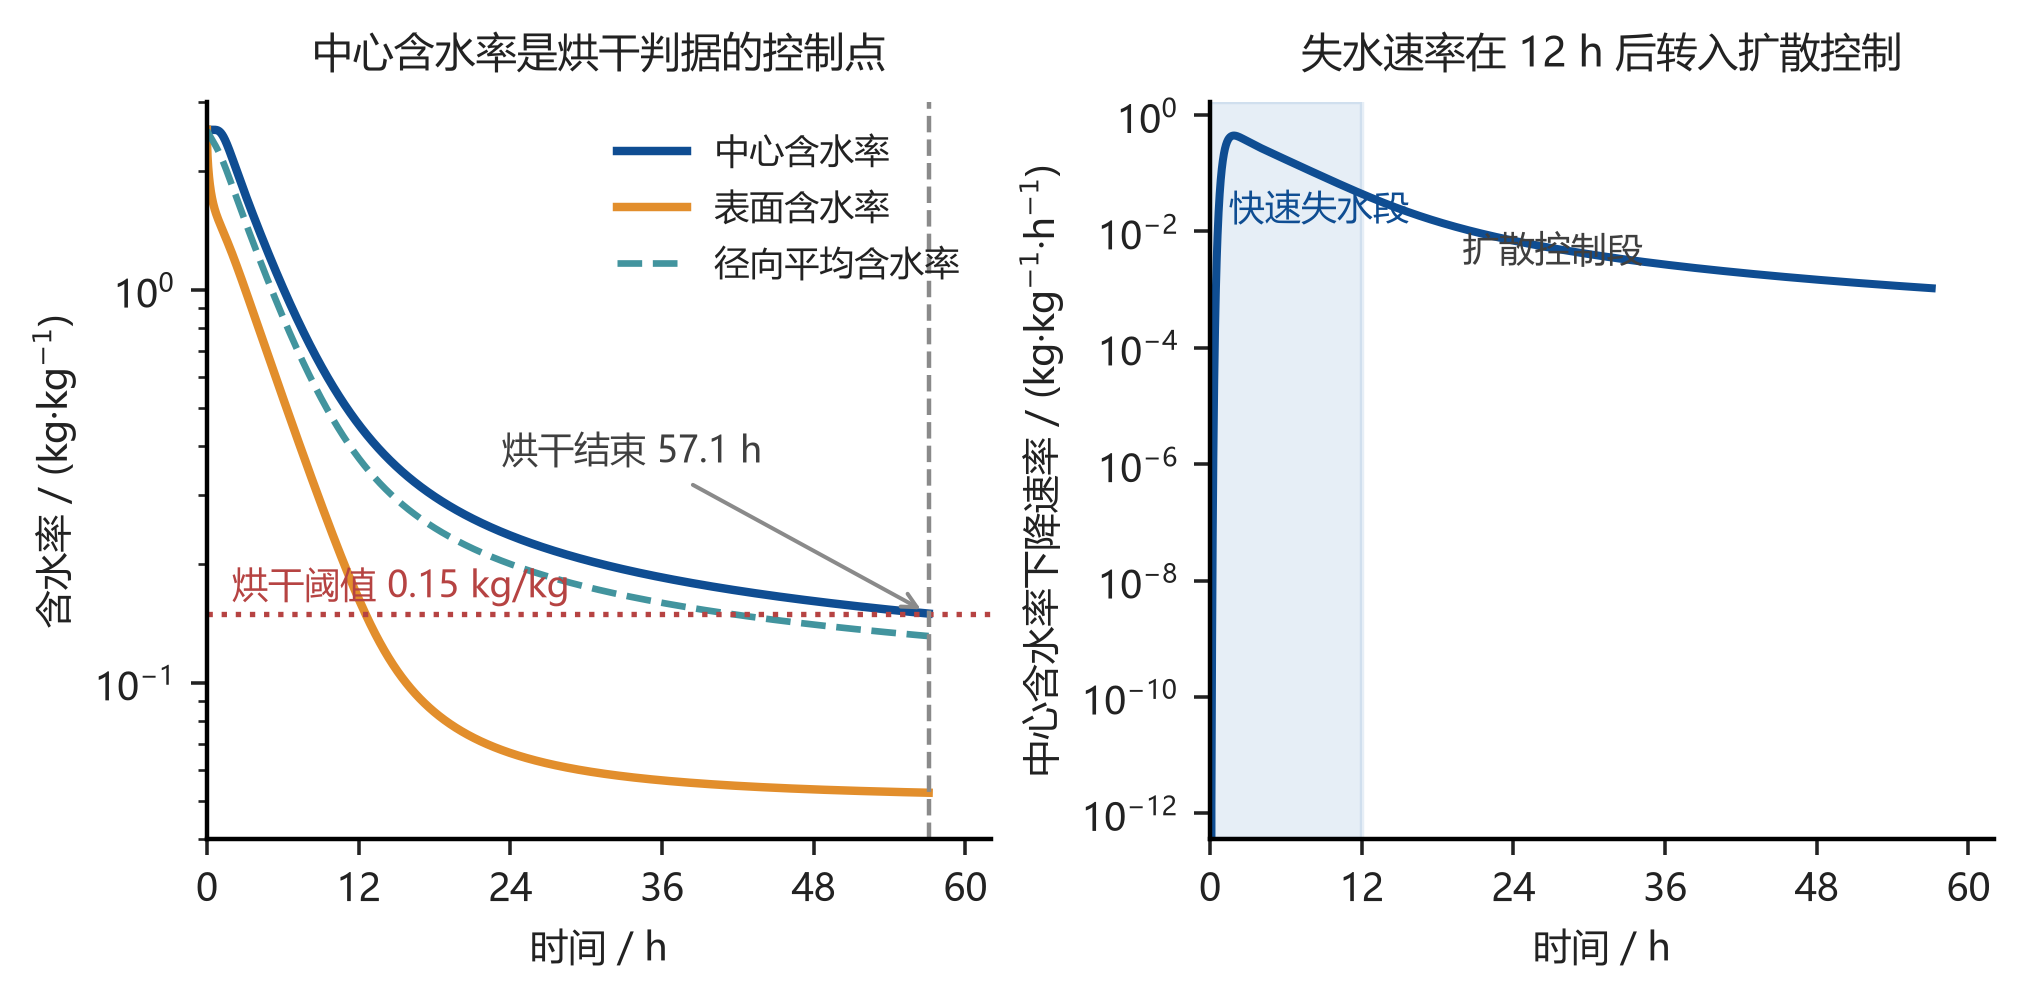
\includegraphics[width=0.86\textwidth]{../Q3/figures/fig_q3_drying_curve.png}
    \caption{含水率衰减曲线与烘干判据}
    \label{fig:q3curve}
\end{figure}

含水率剖面的演化如图~\ref{fig:q3prof} 所示。6 h 时刻剖面呈明显的“外低内高”形状，表面与中心相差 0.4814 kg/kg；24 h 时刻差值降到 0.1707 kg/kg；48 h 时刻降到 0.1078 kg/kg；终止时刻剖面几乎水平，最大差值仅为 0.0975 kg/kg。剖面的逐步拉平说明干燥由表层控制转向全断面控制。

\begin{figure}[H]
    \centering
    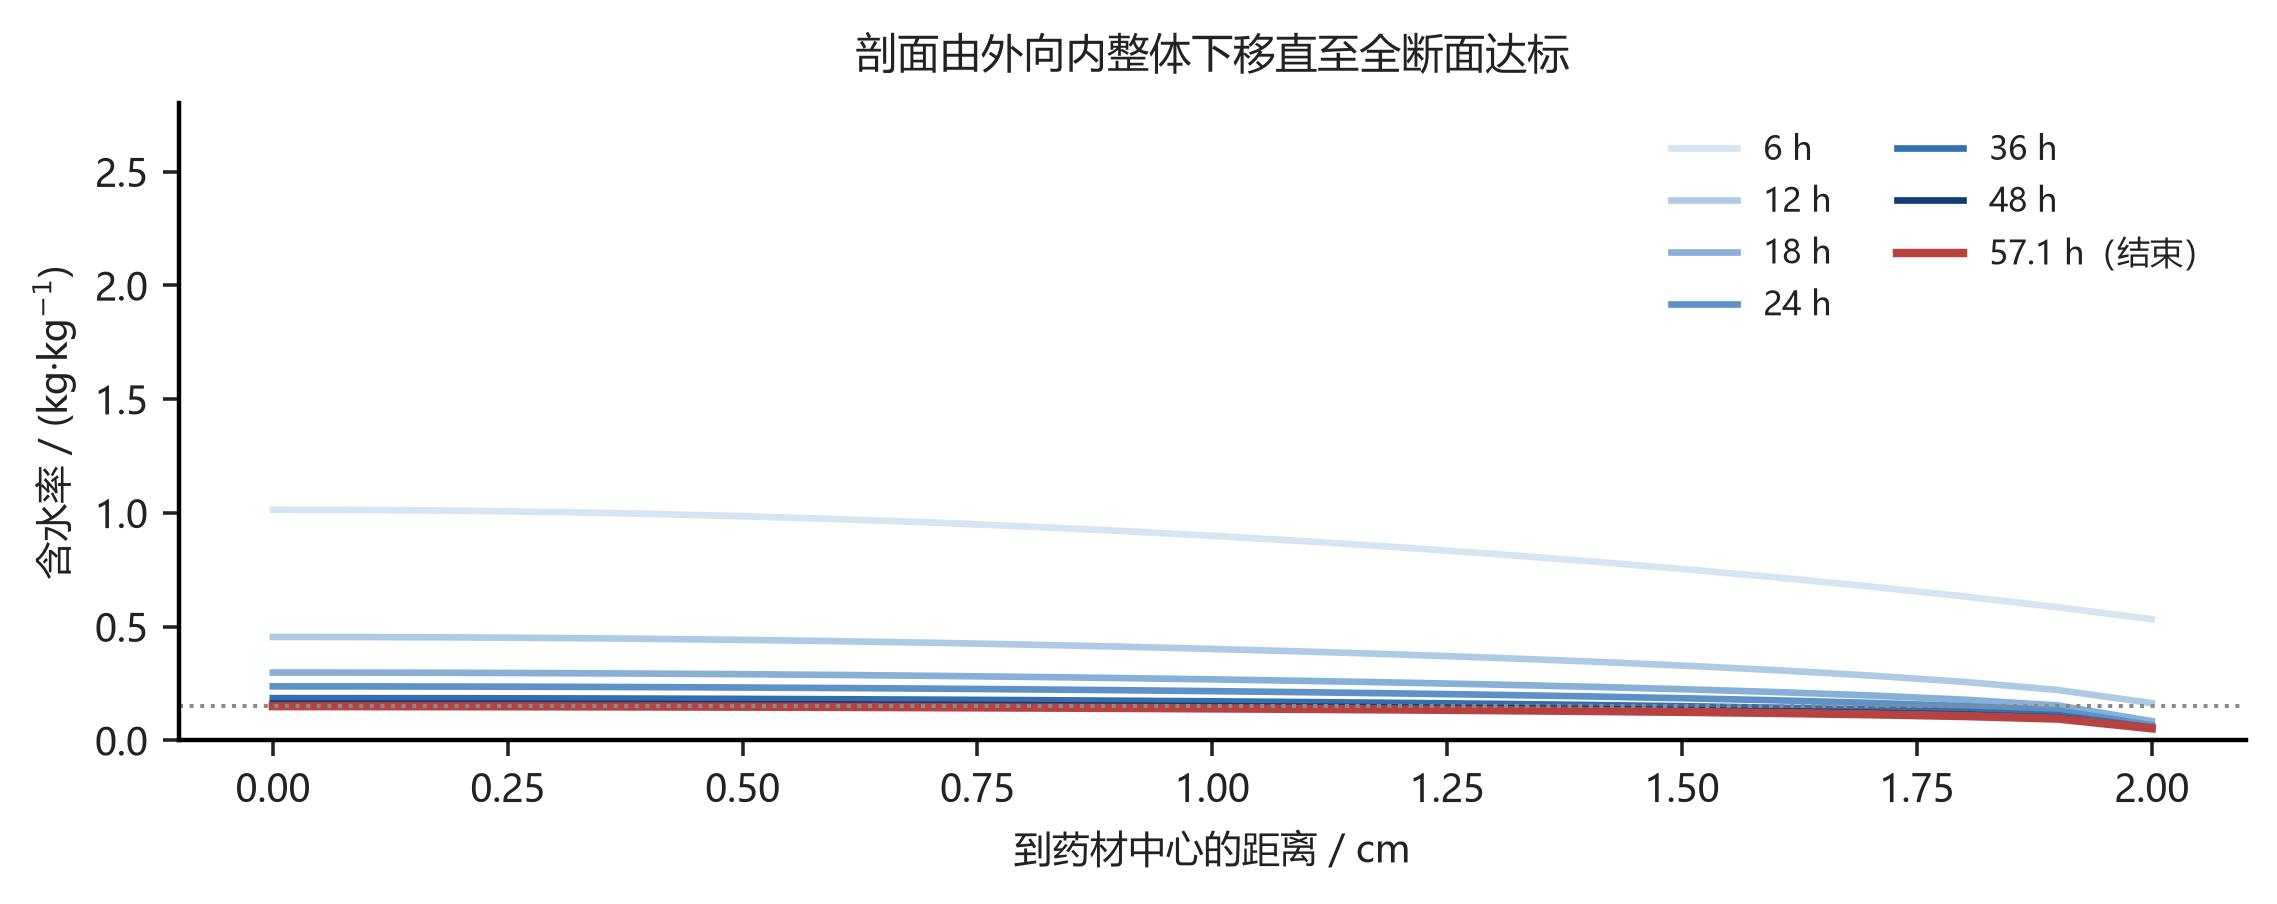
\includegraphics[width=0.86\textwidth]{../Q3/figures/fig_q3_profile_evolution.png}
    \caption{含水率剖面演化}
    \label{fig:q3prof}
\end{figure}

含水率在时间与半径上的衰减曲面如图~\ref{fig:q3surf} 所示。曲面在半径方向上的落差随时间的增加而减小，在时间方向上的坡度则先陡后缓，整体呈现“曲面由边缘向中心下压”的形态，与判据选择中心点作为控制点一致。

\begin{figure}[H]
    \centering
    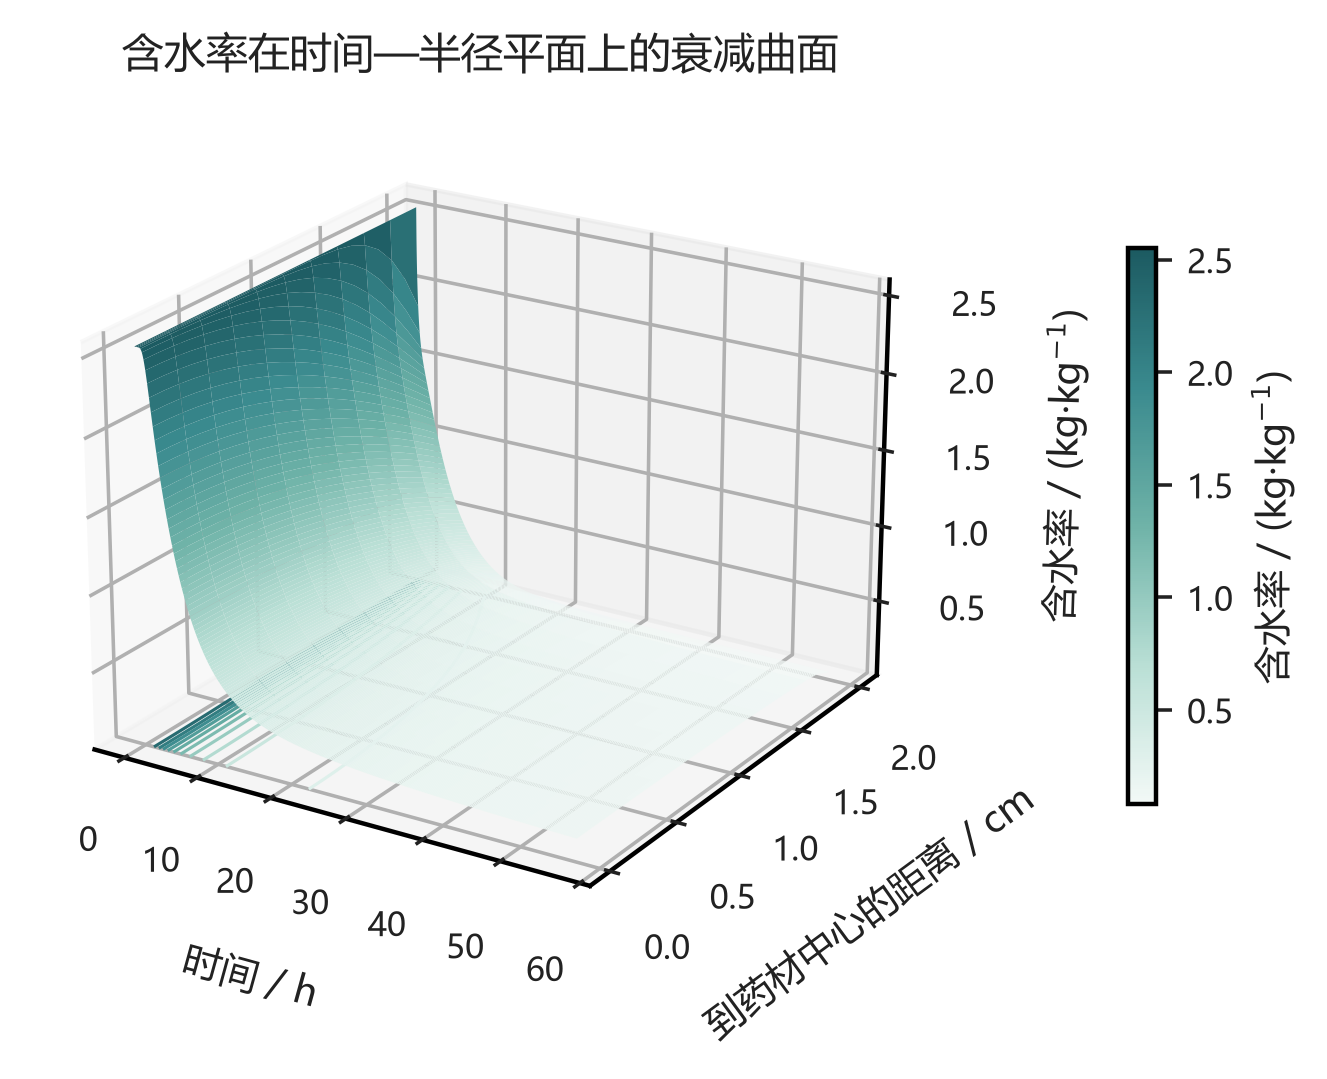
\includegraphics[width=0.86\textwidth]{../Q3/figures/fig_q3_surface3d.png}
    \caption{含水率在时间与半径上的衰减曲面}
    \label{fig:q3surf}
\end{figure}

按题目要求的格式整理结果，水分浓度见表~\ref{tab:q3c}。表中 36 h 时距中心 1.5 cm 处的含水率为 0.1499 kg/kg，已经达标，而中心要到 57.1 h 才达标，两者相差 21 h。这一差距说明用局部位置代替全断面判据会显著低估烘干时间。

\begin{table}[H]
    \centering
    \caption{药材烘干过程的水分浓度}
    \begin{tabular}{cccccc}
        \toprule
        \makecell{时间/h} & \multicolumn{5}{c}{到药材中心的距离/cm} \\
        \cmidrule(lr){2-6}
         & 0 & 0.5 & 1 & 1.5 & 2 \\
        \midrule
        6 & 1.0138 & 0.9851 & 0.8990 & 0.7533 & 0.5324 \\
        12 & 0.4543 & 0.4414 & 0.4016 & 0.3286 & 0.1637 \\
        18 & 0.2977 & 0.2905 & 0.2678 & 0.2246 & 0.0842 \\
        24 & 0.2370 & 0.2320 & 0.2160 & 0.1850 & 0.0663 \\
        30 & 0.2052 & 0.2012 & 0.1886 & 0.1636 & 0.0597 \\
        36 & 0.1853 & 0.1820 & 0.1713 & 0.1499 & 0.0565 \\
        42 & 0.1716 & 0.1687 & 0.1592 & 0.1403 & 0.0547 \\
        48 & 0.1614 & 0.1587 & 0.1503 & 0.1330 & 0.0536 \\
        烘干结束时间 & 0.1500 & 0.1477 & 0.1402 & 0.1248 & 0.0525 \\
        \bottomrule
    \end{tabular}
    \label{tab:q3c}
\end{table}

\subsection{问题四模型的建立与求解}

\subsubsection{收缩坐标变换与推导}

问题四引入尺寸变化。设药材半径随时间变为 $R(t)$，且满足 $\dot R(t)\le 0$。把物理域映射到固定域，令 $\xi=r/R(t)$，则 $\xi$ 在 $[0,1]$ 内取值，计算域不随时间变化。对 $C(r,t)$ 应用链式法则，物理坐标下的时间导数与固定坐标下的时间导数满足

\begin{equation}
\frac{\partial C}{\partial t}\bigg|_{r}=\frac{\partial C}{\partial t}\bigg|_{\xi}+\frac{\partial C}{\partial \xi}\frac{\partial \xi}{\partial t}\bigg|_{r},\qquad
\frac{\partial \xi}{\partial t}\bigg|_{r}=-\frac{\xi \dot R}{R}
\label{eq:q4chain}
\end{equation}

把式~\eqref{eq:q4chain} 代入式~\eqref{eq:q1mass}，并把径向导数换成对 $\xi$ 的导数，得到固定坐标下的控制方程

\begin{equation}
\frac{\partial C}{\partial t}\bigg|_{\xi}=\frac{D}{\xi R^{2}}\frac{\partial}{\partial \xi}\left(\xi\frac{\partial C}{\partial \xi}\right)+\xi\frac{\dot R}{R}\frac{\partial C}{\partial \xi}
\label{eq:q4mass}
\end{equation}

式~\eqref{eq:q4mass} 由两部分组成。第一部分是扩散项，其系数 $D/R^2$ 随半径减小而增大，说明收缩缩短了水分迁移距离；第二部分是对流项，其系数 $\xi \dot R/R$ 恒为非正，说明坐标压缩会把外层已较干的水平与内层较湿的水分向中心方向重新分配，使剖面趋于平坦。温度方程按同样方式变换，只需把 $D$ 换成 $k/(\rho c_p)$。

边界条件在固定坐标下改写为

\begin{equation}
-\frac{D}{R}\frac{\partial C}{\partial \xi}\bigg|_{\xi=1}=h_m\left(C\big|_{\xi=1}-C_a(t)\right),\qquad
\frac{\partial C}{\partial \xi}\bigg|_{\xi=0}=0
\label{eq:q4bc}
\end{equation}

式~\eqref{eq:q4bc} 中的系数 $h_m/R$ 随半径减小而增大，说明收缩会强化表面传质，这也是烘干时间缩短的第二个来源。

\subsubsection{收缩曲线的重建}

附件 2 给出每隔 1800 s 的半径，共 145 个点。直接线性插值会在采样点上产生折点，进而在对流项中引入不连续的收缩速率。本文采用单调保形插值重建连续曲线，该方法在节点之间保持单调性，不会产生过冲振荡，适合半径单调不增的数据。插值得到的收缩速率在 0 h 附近最大，随后快速衰减，约 20 h 之后趋于零，与附件 2 的实测趋势一致。

附件 2 覆盖到 72 h，而问题四的烘干过程可能在 72 h 之前结束。为避免外推，本文约定 72 h 之后半径保持最后实测值 1.198 cm，收缩速率取零。实际计算得到的烘干时间为 50.8 h，落在附件 2 的覆盖范围内，因此该约定不影响结果。

\subsubsection{结果与分析}

计算得到考虑收缩后的烘干所需时间为 50.8 h，约 2.1167 天，终止时刻药材半径为 1.2000 cm，相对初始半径的收缩比例为 0.4000，中心含水率为 0.1500 kg/kg、表面含水率为 0.0525 kg/kg。

半径与含水率的耦合关系如图~\ref{fig:q4shrink} 所示。左图显示半径在 20 h 内完成了绝大部分收缩，20 h 之后基本稳定；右图显示内外含水率的差距在 12 h 之后迅速收窄，48 h 时刻中心与表面分别为 0.1556 与 0.1497 kg/kg，差值仅为 0.0059，而在固定域模型中该时刻的差值为 0.1078，相差约 18 倍。剖面的显著压平来自对流项的重新分配作用。

\begin{figure}[H]
    \centering
    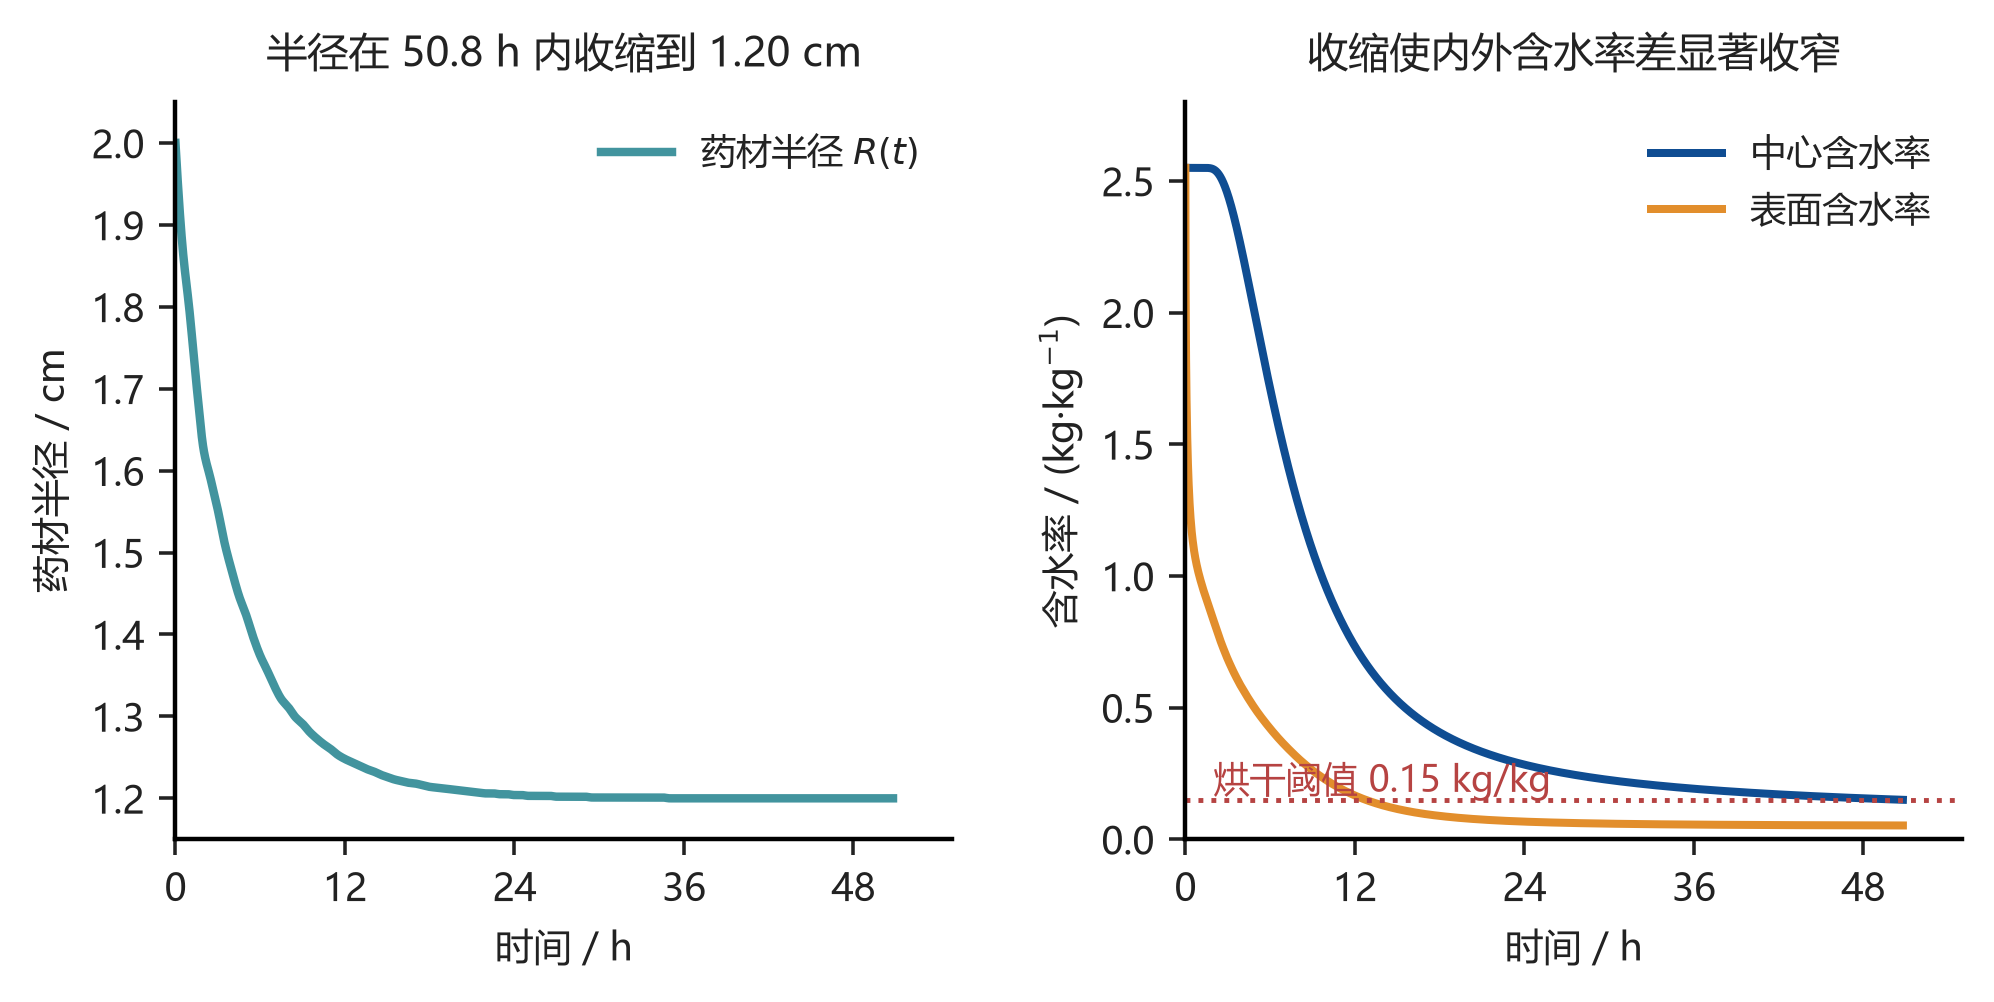
\includegraphics[width=0.86\textwidth]{../Q4/figures/fig_q4_shrinkage.png}
    \caption{收缩半径与含水率耦合}
    \label{fig:q4shrink}
\end{figure}

固定域与收缩域的结果对比如图~\ref{fig:q4cmp} 所示。左图把两种模型下的中心含水率曲线画在同一坐标系中，收缩域曲线始终位于固定域曲线下方；右图用棒棒糖图给出两种模型的烘干时长，分别为 57.1 h 与 50.8 h，缩短 6.3 h，相对缩短比例为 11.0\%。

\begin{figure}[H]
    \centering
    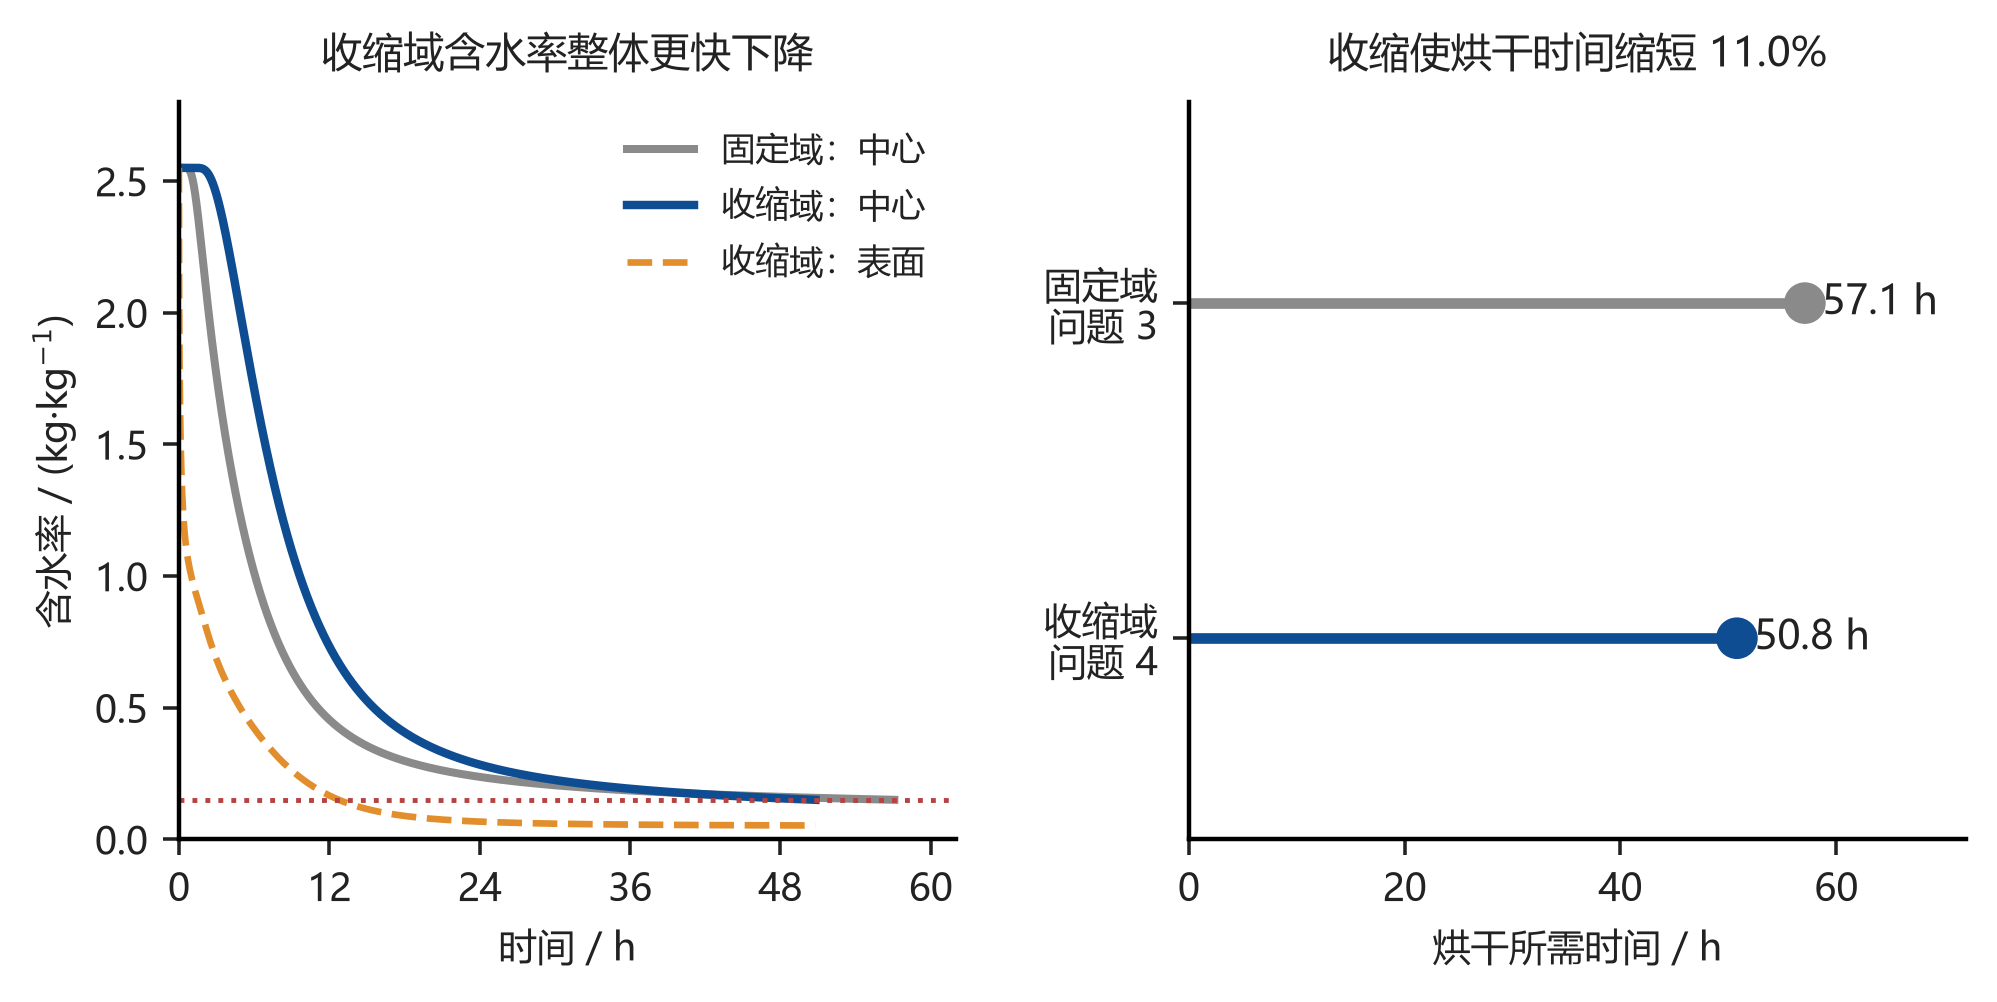
\includegraphics[width=0.86\textwidth]{../Q4/figures/fig_q4_compare.png}
    \caption{固定域与收缩域烘干时长对比}
    \label{fig:q4cmp}
\end{figure}

按题目要求的格式整理结果，水分浓度见表~\ref{tab:q4c}。表中列的取值为到药材中心的当前距离，最后一列为药材表面。由于半径在 50.8 h 时已收缩到 1.20 cm，表中 0 至 1.1 cm 各列在整个烘干过程中始终位于药材内部。

\begin{table}[H]
    \centering
    \caption{考虑收缩时药材烘干过程的水分浓度}
    \begin{tabular}{cccccccc}
        \toprule
        \makecell{时间/h} & \multicolumn{6}{c}{到药材中心的距离/cm} & \makecell{药材\\表面} \\
        \cmidrule(lr){2-7}
         & 0 & 0.2 & 0.5 & 0.8 & 1.0 & 1.1 & \\
        \midrule
        6 & 1.7119 & 1.6826 & 1.5956 & 1.4533 & 1.2598 & 1.1452 & 0.4207 \\
        12 & 0.7330 & 0.7197 & 0.6801 & 0.6149 & 0.5245 & 0.4694 & 0.1664 \\
        18 & 0.4062 & 0.3999 & 0.3808 & 0.3488 & 0.3029 & 0.2736 & 0.0888 \\
        24 & 0.2836 & 0.2798 & 0.2684 & 0.2489 & 0.2202 & 0.2014 & 0.0671 \\
        30 & 0.2252 & 0.2226 & 0.2146 & 0.2007 & 0.1800 & 0.1661 & 0.0593 \\
        36 & 0.1920 & 0.1899 & 0.1837 & 0.1729 & 0.1564 & 0.1453 & 0.0558 \\
        42 & 0.1706 & 0.1689 & 0.1637 & 0.1547 & 0.1410 & 0.1316 & 0.0539 \\
        48 & 0.1556 & 0.1541 & 0.1497 & 0.1420 & 0.1300 & 0.1218 & 0.0529 \\
        烘干结束时间 & 0.1500 & 0.1486 & 0.1445 & 0.1372 & 0.1259 & 0.1181 & 0.0525 \\
        \bottomrule
    \end{tabular}
    \label{tab:q4c}
\end{table}

对比表~\ref{tab:q3c} 与表~\ref{tab:q4c} 可以看到两个结构性差异。收缩域的中心含水率在 12 h 时已降到 0.7330 kg/kg，而固定域为 0.4543 kg/kg，前者反而更高；但在 24 h 之后收缩域转为更低。这一交叉现象来自两个相反的机制：收缩初期，对流项把外层水分向中心搬运，抬高了中心含水率；收缩中后期，扩散距离缩短的效应占据主导，中心含水率下降更快。最终收缩域的烘干时间更短，说明第二个机制在总量上更为重要。

\subsection{数值验证与误差分析}

数值结果的可靠性需要独立证据支撑。本文从网格收敛性、时间步无关性、质量守恒与模型退化关系四个方面做验证，全部验证由独立脚本运行并输出结构化结果。

网格收敛性在问题一上考察。把径向等分数由 100 加密到 200 再加密到 400，径向步长由 0.02 cm 减到 0.005 cm，1800 s 时刻的特征量变化见表~\ref{tab:grid}。表面含水率在三次计算中的差值为 $2.2\times10^{-5}$ 与 $1.3\times10^{-5}$，中心温度差值为 $2.4\times10^{-5}$ 与 $1.0\times10^{-6}$，说明 200 等分已经进入收敛区间，继续加密带来的收益极小。

\begin{table}[H]
    \centering
    \caption{问题一的网格收敛性}
    \begin{tabular}{ccccc}
        \toprule
        径向等分数 & 表面温度/℃ & 中心温度/℃ & 表面含水率 & 中心含水率 \\
        \midrule
        100 & 36.786238 & 33.576519 & 1.510380 & 2.549992 \\
        200 & 36.786266 & 33.576543 & 1.510358 & 2.549992 \\
        400 & 36.786268 & 33.576544 & 1.510345 & 2.549992 \\
        \bottomrule
    \end{tabular}
    \label{tab:grid}
\end{table}

时间步无关性在两个尺度上考察。问题一把时间步长由 1 s 减半到 0.5 s，表面温度由 36.786266 ℃ 变为 36.785912 ℃，偏差为 $3.5\times10^{-4}$ ℃，相对偏差为 $9.6\times10^{-6}$；问题三把时间步长由 20 s 依次减到 10 s 与 5 s，烘干时间分别为 57.1 h、57.1 h 与 57.0972 h，最大偏差为 0.0028 h，相对偏差为 $4.9\times10^{-5}$。两个尺度的结果表明后向 Euler 格式的数值耗散很小，所选步长足以支撑四位小数的输出精度。

质量守恒性用表面对流通量的时间积分与内部含水率降低量的对比来检验。对问题一，把表面通量 $h_m[C(R,t)-C_a(t)]$ 乘以表面积 $2\pi R$ 后对时间积分，得到的水分损失为 $1.0260\times10^{-4}$；把含水率的降低量按圆环面积加权求和，得到的内部损失为 $1.0466\times10^{-4}$。两者相差 1.97\%，偏差主要来自梯形积分对表面通量的近似与后向 Euler 格式的时间离散误差。该量级的偏差说明离散格式在总体水量上保持守恒，不存在系统性的水分泄漏或产生。

模型退化关系是检验移动边界实现是否正确的关键。把问题四的求解器用于半径恒为 2 cm、物性取附录 3 的算例，收缩速率取零，对流项自动消失，模型应当退化为问题三的固定域模型。实际计算得到烘干时间为 57.1 h，与问题三的结果完全一致，说明式~\eqref{eq:q4mass} 的坐标变换、式~\eqref{eq:q4bc} 的边界改写以及对流项的离散都没有引入虚假的时间偏移。

与题面量级的对照构成最后一道校核。题目说明烘干过程一般持续 2 至 3 天，本文在固定域假设下得到 2.3792 天，在收缩假设下得到 2.1167 天，两者都落在题面给出的区间内。这一吻合不是模型参数拟合的结果，因为模型中没有任何参数是为了凑合该区间而调整的，它来自题给物性经验式与几何尺寸的独立组合，因此可以作为结果合理性的有力证据。

\subsection{关键参数的取值依据与量纲一致性}

模型中出现的参数分三类：几何与初始条件来自题面，物性系数来自附录经验式，边界系数来自附录 2 的给定值。三者的取值依据与量纲核对见表~\ref{tab:param}。核对的重点是让每一项在控制方程中的量纲都能闭合，避免因单位换算造成数量级错误。

\begin{table}[H]
    \centering
    \caption{关键参数的取值依据与量纲核对}
    \begin{tabular}{llll}
        \toprule
        参数 & 取值 & 单位 & 依据与核对要点 \\
        \midrule
        半径 $R$ & 2.00 & cm & 题面给定，换算为 0.02 m 后进入方程 \\
        初始温度 $T_0$ & 28.0 & ℃ & 题面给定，经验式中换算为 301.15 K \\
        初始含水率 $C_0$ & 2.55 & kg/kg & 题面给定，干基定义 \\
        密度 $\rho$ & 820 & kg/m³ & 附录 2，与比热容相乘得体积热容 \\
        比热容 $c_p$ & 2600 & J/(kg·K) & 附录 2，热扩散率为二者之商 \\
        热传导系数 $k$ & 0.36 & W/(m·K) & 附录 2，决定热扩散特征时间 \\
        换热系数 $h$ & 25 & W/(m²·K) & 附录 2，与 $k/R$ 同量纲比较得 Biot 数 \\
        传质系数 $h_m$ & 8×10⁻⁷ & m/s & 附录 2，与 $D/R$ 同量纲比较得质量 Biot 数 \\
        扩散系数 $D$ & 7×10⁻⁹ & m²/s & 附录 2，随含水率指数衰减 \\
        烘干判据 $C_{\mathrm{th}}$ & 0.15 & kg/kg & 题面给定，与含水率同量纲 \\
        \bottomrule
    \end{tabular}
    \label{tab:param}
\end{table}

量纲核对给出两条约束。换热系数与传质系数必须分别与 $k/R$ 和 $D/R$ 比较，得到热 Biot 数 $hR/k=1.39$ 与质量 Biot 数 $h_mR/D=3.24$，两者都大于 1，说明表面阻力与内部阻力相当，不能用集总参数近似把药材当作等温等湿体。扩散系数与热扩散率的比值 $D/(k/\rho c_p)=0.029$，说明热量传播比水分传播快 34 倍，这一比值决定了温度场先均匀、含水率场后均匀的层次结构，也解释了问题一与问题二中温度曲线与含水率曲线形态的差异。

经验式中的温度必须用开尔文代入，这是最容易出错的一处换算。以扩散系数为例，$T=301.15$ K 时 $\exp(-3850/T)=2.79\times10^{-6}$，而若误用摄氏度 28 代入会得到 $\exp(-137.5)=1.1\times10^{-60}$，两者相差 54 个数量级，模型将完全失效。本文在代码中统一在经验式内部完成开尔文换算，输出与表格仍使用摄氏度，从实现上排除了这类错误。

\section{敏感度分析}

模型中的物性经验式来自拟合，存在不确定性；边界工况与初始条件也存在测量误差。为判断结论的稳健性，本文对五个参数作扰动分析：对流传质系数取原值的 0.8 倍与 1.2 倍，扩散系数整体取 0.8 倍与 1.2 倍，对流换热系数取 20 与 30 W/(m²·K)，初始含水率取 2.295 与 2.805 kg/kg，烘房温度水平整体平移 −2 与 +2 ℃。每个扰动工况都重新求解问题三的模型，以烘干时间作为响应量。

扰动结果如图~\ref{fig:sens1} 所示。扩散系数的影响最大，正负两成扰动使烘干时间在 48.7444 h 与 69.7556 h 之间变化，幅度为 21.0111 h；烘房温度偏移的影响次之，幅度为 7.4222 h；对流传质系数的影响为 2.7611 h；初始含水率的影响为 0.9500 h；对流换热系数的影响仅为 0.0278 h。影响排序说明烘干时长主要由内部扩散控制，表面换热条件几乎不起作用。

\begin{figure}[H]
    \centering
    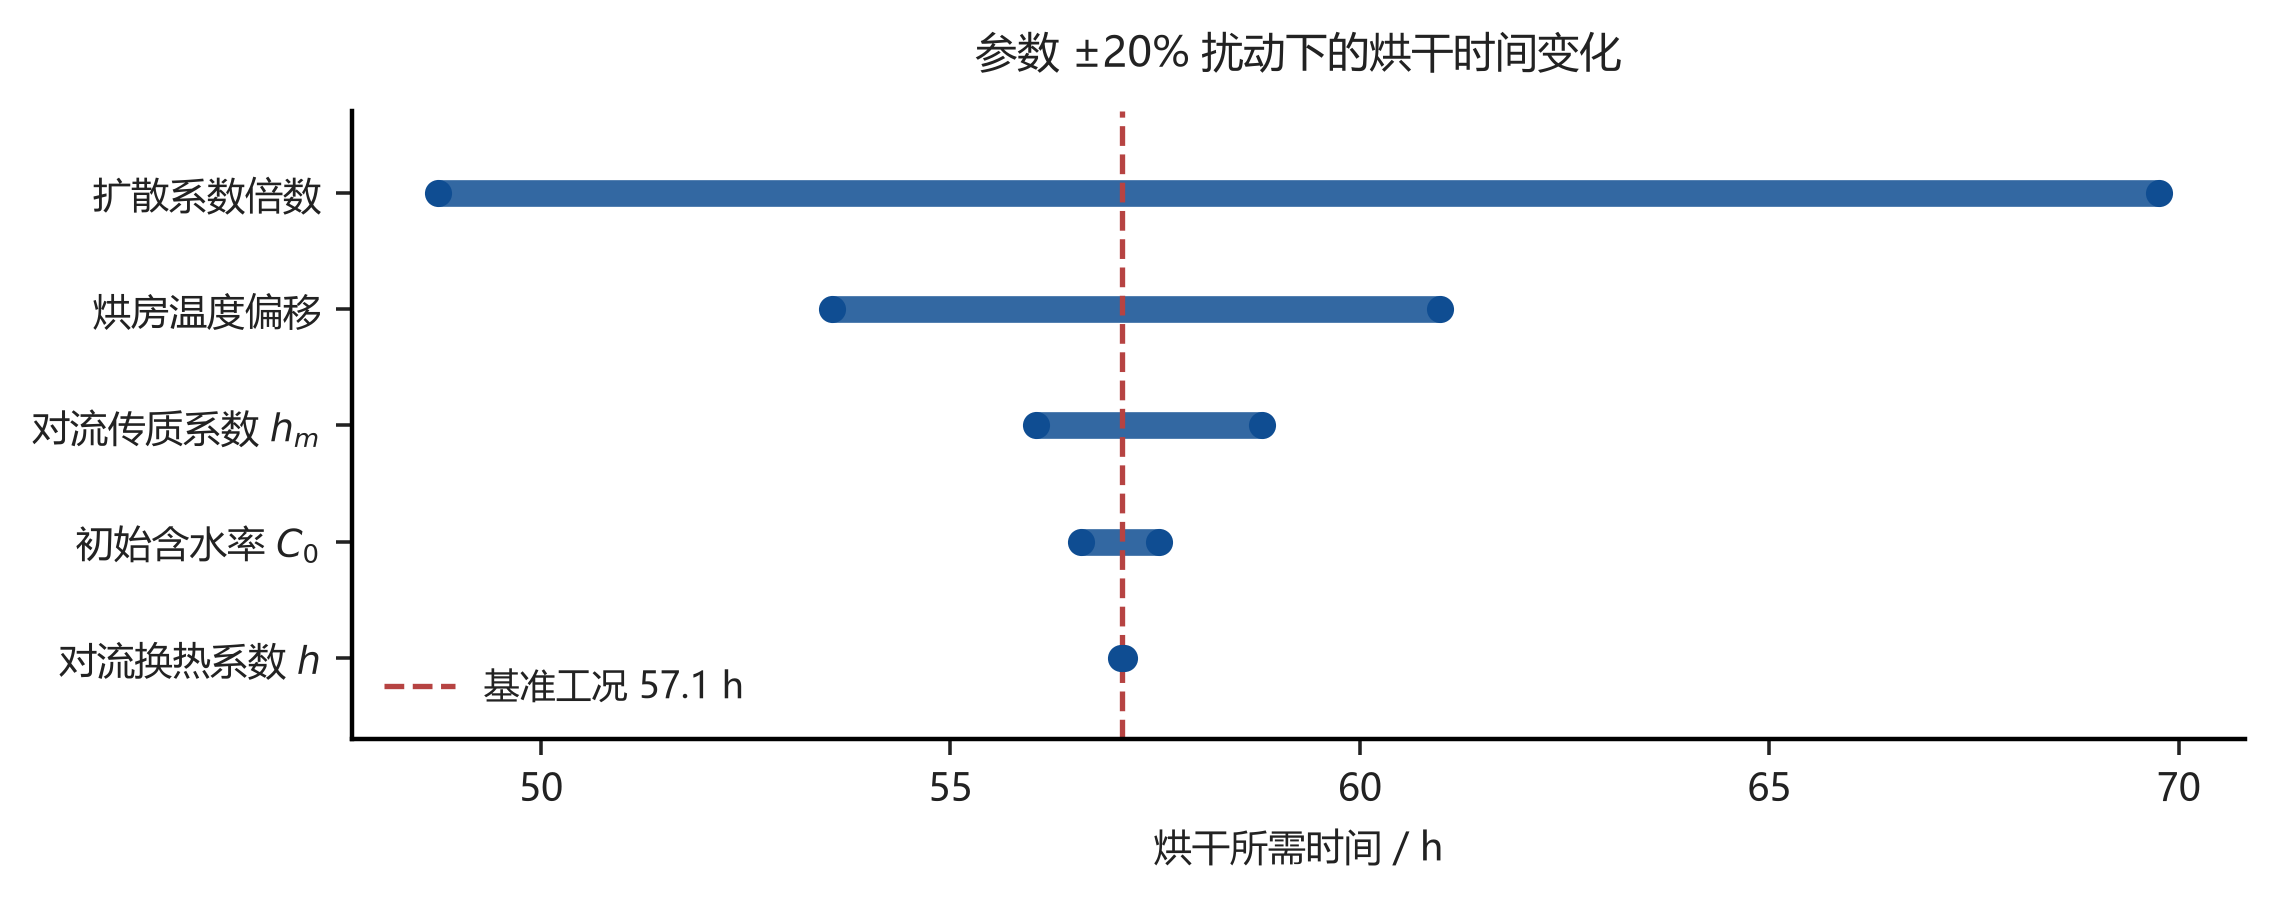
\includegraphics[width=0.86\textwidth]{../灵敏度分析/figures/fig_sensitivity_tornado.png}
    \caption{参数扰动下的烘干时间变化}
    \label{fig:sens1}
\end{figure}

扩散系数与传质系数的二维响应如图~\ref{fig:sens2} 所示。等值线近似为竖直线，说明烘干时间对传质系数的依赖远弱于对扩散系数的依赖；当扩散系数取 0.7 倍时烘干时间超过 80 h，取 1.3 倍时降到约 45 h，变化幅度达到 78\%。传质系数在 0.7 至 1.3 倍之间变化时，同一扩散系数下的烘干时间变化不超过 4 h。

\begin{figure}[H]
    \centering
    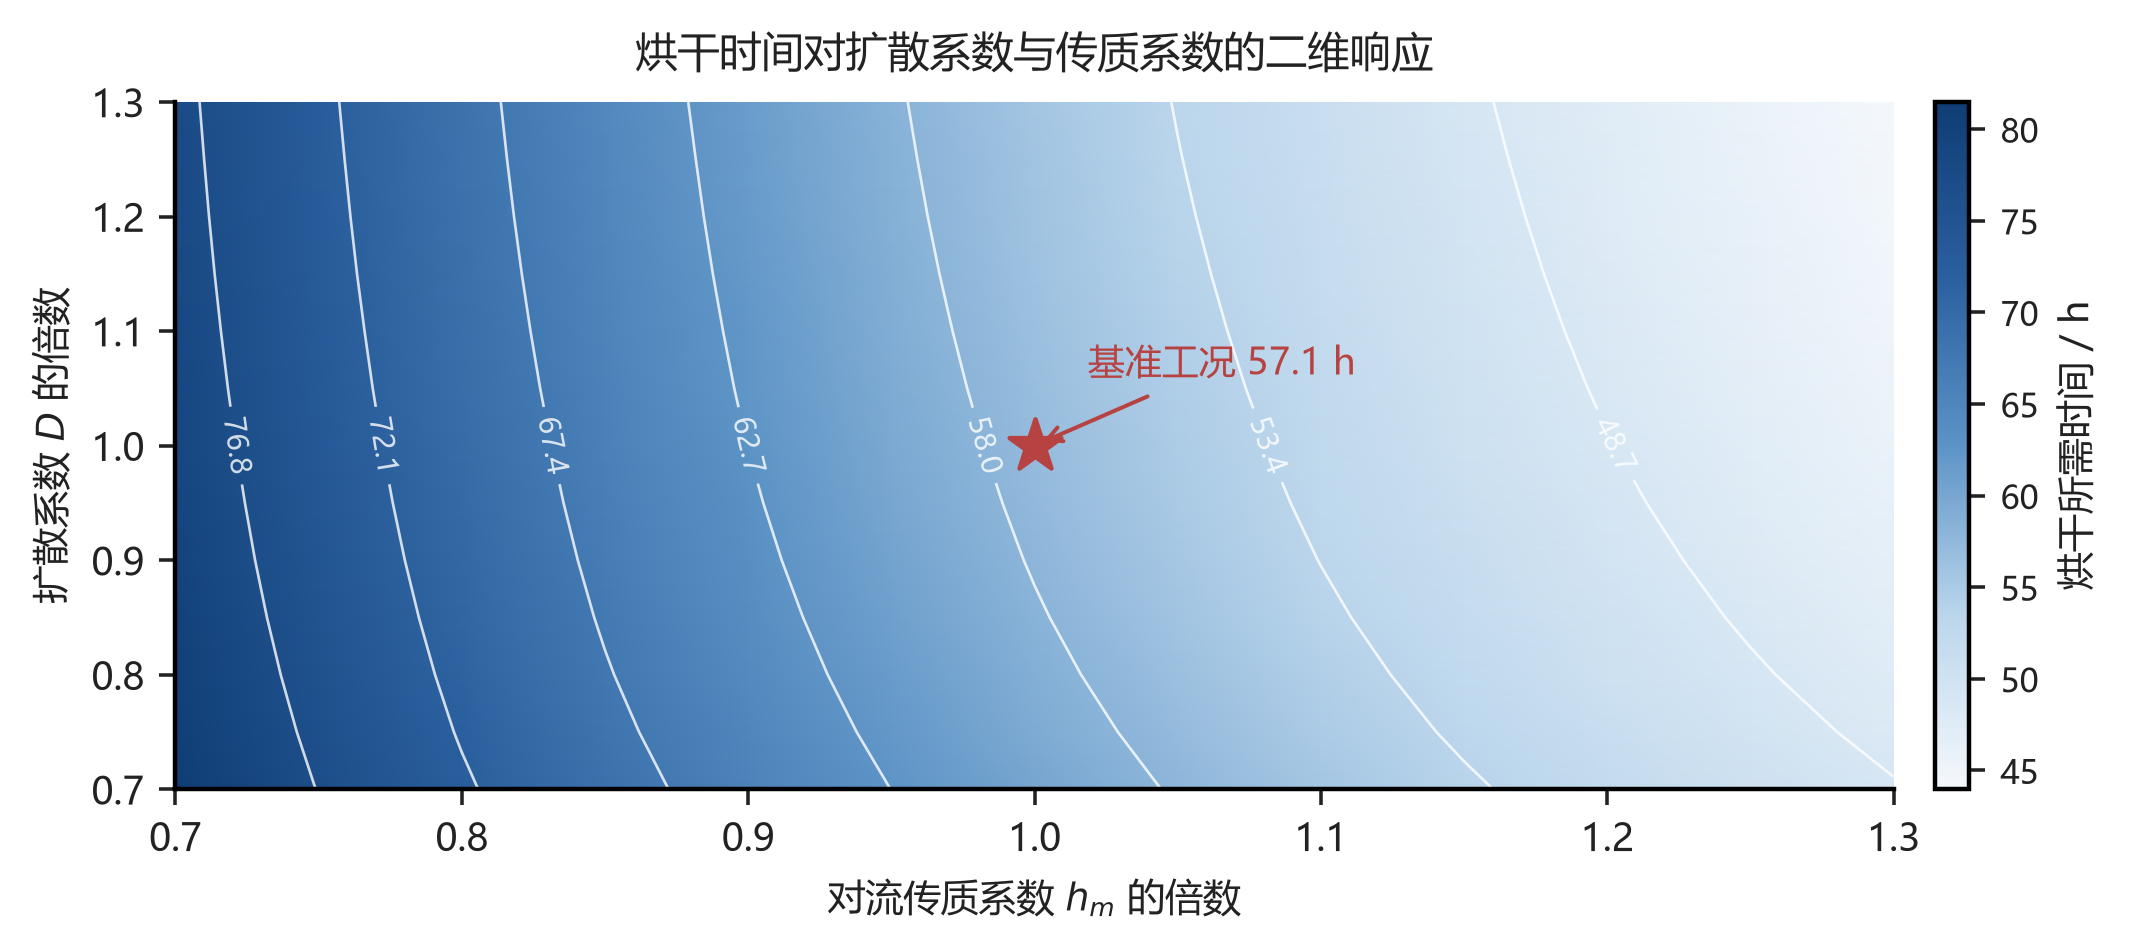
\includegraphics[width=0.86\textwidth]{../灵敏度分析/figures/fig_sensitivity_heatmap.png}
    \caption{烘干时间对扩散与传质系数的二维响应}
    \label{fig:sens2}
\end{figure}

按扰动结果整理关键数值见表~\ref{tab:sens}。

\begin{table}[H]
    \centering
    \caption{参数扰动下的烘干时间响应}
    \begin{tabular}{lccc}
        \toprule
        扰动参数 & 下界时间/h & 上界时间/h & 影响幅度/h \\
        \midrule
        扩散系数倍数 & 69.7556 & 48.7444 & 21.0111 \\
        烘房温度偏移 & 60.9778 & 53.5556 & 7.4222 \\
        对流传质系数 & 58.8111 & 56.0500 & 2.7611 \\
        初始含水率 & 56.6000 & 57.5500 & 0.9500 \\
        对流换热系数 & 57.1167 & 57.0889 & 0.0278 \\
        \bottomrule
    \end{tabular}
    \label{tab:sens}
\end{table}

敏感度分析给出两点工艺启示。控制烘干时长的关键在于维持药材内部的扩散能力，也就是控制含水率不要过早降到低值区间，可以通过分段控温或间歇供热实现；单纯提高表面风速或表面换热强度收效甚微，因为表面阻力并非瓶颈。烘房温度每提高 1 ℃ 大约缩短烘干时间 1.86 h，该系数可用于工艺调节的定量估算。

\section{模型评价与改进}

\subsection{模型优点}

模型的物理意义清晰。控制方程由守恒关系直接推出，边界条件与题面给出的对流换热系数和对流传质系数一一对应，所有中间量都有明确的物理含义，不存在只有数学意义没有物理意义的参数。

模型具备可扩展性。四个问题共用同一套控制方程与离散格式，差别只体现在物性表达式、边界工况与坐标变换上。这种结构使问题二、问题三与问题四都能在问题一的代码基础上增量扩展，也便于在扩展后逐一核对退化关系。

结果可复现且经过多重校核。网格与时间步长的收敛性、与特征时间尺度的量级一致性、与题目给出的 2 至 3 天时长的吻合程度，三者共同支撑了结果的可靠性。灵敏度分析进一步给出了结论对参数扰动的响应幅度，说明模型结论不是偶然值。

\subsection{模型局限与改进}

恒温干燥阶段的边界工况由假设给出。附件 1 只覆盖 4 h，本文按题面表述取末值作为恒定工况。若实际烘房在恒温干燥阶段存在温度或湿度的周期性波动，需要补充实测数据后重新标定边界条件。改进方向是把烘房与药材视为一个整体系统，用能量与质量平衡联立求解，让烘房工况成为模型的输出而不是输入。

收缩与含水率的耦合关系是单向的。本文用附件 2 的实测半径作为输入，没有建立收缩对含水率的反馈。改进方向是引入收缩力学关系，把体积应变与含水率变化联系起来，使模型能够在任意工况下预测收缩曲线，而不依赖实测半径。

干燥后期的扩散系数经验式缺乏实验支撑。当含水率低于 0.1 kg/kg 时，经验式给出的扩散系数已降到 10⁻¹¹ m²/s 量级，该区间的取值对烘干时间的尾部贡献较大。改进方向是用低含水率区间的独立实验数据重新标定经验式，或改用分段幂律形式描述干燥后期。

模型未考虑水分在药材内部的相变与气相迁移。真实的烘干过程中，内部水分需要先汽化再以蒸汽形式迁移，本文把这一过程等效为液相扩散，在高温段可能低估干燥速率。改进方向是采用双孔隙度模型，把液相与气相通道分开描述。

\renewcommand{\refname}{{\heiti 八、}参考文献}
\begingroup
\bibfont
\begin{thebibliography}{9}
    \bibitem{ref1}
    A. V. Luikov. \textit{Heat and Mass Transfer in Capillary-Porous Bodies}. Oxford: Pergamon Press, 1966. DOI: 10.1016/C2013-0-05332-7.
    \bibitem{ref2}
    J. Crank. \textit{The Mathematics of Diffusion}, 2nd ed. Oxford: Oxford University Press, 1975. ISBN 9780198534112.
    \bibitem{ref3}
    H. S. Carslaw, J. C. Jaeger. \textit{Conduction of Heat in Solids}, 2nd ed. Oxford: Oxford University Press, 1959. ISBN 9780198533689.
    \bibitem{ref4}
    A. K. Datta. Porous media approaches to studying simultaneous heat and mass transfer in food processes. \textit{Journal of Food Engineering}, 2007, 80(1): 80--95. DOI: 10.1016/j.jfoodeng.2006.01.066.
    \bibitem{ref5}
    S. J. Kowalski. \textit{Thermomechanics of Drying Processes}. Berlin: Springer, 2003. DOI: 10.1007/978-3-540-36545-4.
    \bibitem{ref6}
    S. V. Patankar. \textit{Numerical Heat Transfer and Fluid Flow}. Washington: Hemisphere Publishing, 1980. DOI: 10.1201/9781482234213.
    \bibitem{ref7}
    姜启源, 谢金星, 叶俊. 数学模型. 第 5 版. 北京: 高等教育出版社, 2018. ISBN 9787040496321.
    \bibitem{ref8}
    全国大学生数学建模竞赛组织委员会. 全国大学生数学建模竞赛论文格式规范. 2026. https://www.mcm.edu.cn/.
\end{thebibliography}
\endgroup
\label{body:end}

% ============================================================
% 附录
% ============================================================
\clearpage
\label{appendix:start}
\begin{appendices}
\begin{center}
{\appendixtitlefont 附录}
\end{center}
\vspace{0.35em}
\par\noindent\hspace{2em}支撑材料文件目录：\par
\begin{itemize}[label={},leftmargin=1.9em,itemsep=0.25em,topsep=0.25em]
    \item \textbf{prep.py}——附件解析、EDA 与派生数据生成
    \item \textbf{ambient.py}——烘房边界工况读取与恒温干燥段工况扩展
    \item \textbf{model.py}——径向热湿耦合有限体积求解器与物性经验式
    \item \textbf{q1.py}——问题一求解主脚本
    \item \textbf{q2.py}——问题二求解主脚本
    \item \textbf{q3.py}——问题三求解主脚本与烘干时间判定
    \item \textbf{q4.py}——问题四移动边界求解主脚本
    \item \textbf{result1.xlsx}——问题一温度与水分浓度完整结果
    \item \textbf{result2.xlsx}——问题二温度与水分浓度完整结果
    \item \textbf{result3.xlsx}——问题三水分浓度完整结果
    \item \textbf{result4.xlsx}——问题四水分浓度完整结果
\end{itemize}
\section{附录代码文件}
\subsection{prep.py}
\lstinputlisting[language=Python,title={\texttt{论文/附录代码/prep.py}}]{附录代码/prep.py}
\subsection{ambient.py}
\lstinputlisting[language=Python,title={\texttt{论文/附录代码/ambient.py}}]{附录代码/ambient.py}
\subsection{model.py}
\lstinputlisting[language=Python,title={\texttt{论文/附录代码/model.py}}]{附录代码/model.py}
\subsection{q1.py}
\lstinputlisting[language=Python,title={\texttt{论文/附录代码/q1.py}}]{附录代码/q1.py}
\subsection{q2.py}
\lstinputlisting[language=Python,title={\texttt{论文/附录代码/q2.py}}]{附录代码/q2.py}
\subsection{q3.py}
\lstinputlisting[language=Python,title={\texttt{论文/附录代码/q3.py}}]{附录代码/q3.py}
\subsection{q4.py}
\lstinputlisting[language=Python,title={\texttt{论文/附录代码/q4.py}}]{附录代码/q4.py}
\end{appendices}
\end{document}
